\documentclass[pdftex,dvipsnames]{dissertation}

% --- Encoding stuff ----------------------------------------------------------
% \usepackage[utf8]{inputenc}
\usepackage[T1]{fontenc}

% --- English stuff -----------------------------------------------------------
\usepackage[french,english]{babel}
% \usepackage[english]{babel}
\selectlanguage{english}

\usepackage{xspace}
\usepackage{csquotes}

% --- Debug stuff -------------------------------------------------------------
\usepackage{morewrites} % workaround for "no room for new \write" error

% --- Font stuff --------------------------------------------------------------
\usepackage{stackengine} % for overlapping text

% --- Page formatting ---------------------------------------------------------
\usepackage{multicol}

% --- Appendices --------------------------------------------------------------

% --- Blind text --------------------------------------------------------------
% \usepackage{blindtext} % provide \blindtext, \Blindtext
\usepackage{lipsum}

\usepackage{xargs}   % Use more than one optional parameter in a new commands
% \usepackage{xcolor}  % Coloured text etc.
% \usepackage{pygmentize}

% --- TODO notes --------------------------------------------------------------
\usepackage[loadshadowlibrary,colorinlistoftodos,prependcaption,textsize=small,shadow]{todonotes}
% my alias
\newcommand{\itodo}[1]{\todo[inline]{#1}\PackageWarning{TODO ::}{#1}}
\newcommand{\miss}[1]{\todo[inline,backgroundcolor=white,bordercolor=black]{#1}\PackageWarning{TODO ::}{#1}}
\newcommandx{\unsure}[2][1=]{\todo[linecolor=red,backgroundcolor=red!25,bordercolor=red,#1]{#2}\PackageWarning{TODO ::}{#2!}}
\newcommandx{\change}[2][1=]{\todo[linecolor=blue,backgroundcolor=blue!25,bordercolor=blue,#1]{#2}\PackageWarning{TODO ::}{#2!}}
\newcommandx{\info}[2][1=]{\todo[linecolor=OliveGreen,backgroundcolor=OliveGreen!25,bordercolor=OliveGreen,#1]{#2}\PackageWarning{TODO ::}{#2!}}
\newcommandx{\plus}[2][1=]{\todo[linecolor=Plum,backgroundcolor=Plum!25,bordercolor=Plum,#1]{#2}\PackageWarning{TODO ::}{#2!}}

% --- Symbols, Units and Icons ------------------------------------------------
% \usepackage{fontawesome5} % fontawesomeicons
\usepackage{arydshln} % provide dashline
\usepackage{pifont}% http://ctan.org/pkg/pifont
\usepackage{gensymb} % provide \degree

% --- Math --------------------------------------------------------------------
\usepackage{kmath} % cool delimiters
\usepackage{dsfont} % double stroke
\usepackage[mathscr]{euscript}
\usepackage{xfrac} % provide \sfrac, cool fractions
\usepackage{siunitx}    % provide \ang and SI units
\usepackage{epsdice} % provide \epsdice

% --- Theorem environment------------------------------------------------------
\usepackage{amsthm}
\usepackage{thmtools}
\usepackage{thm-restate}
\declaretheorem[%
    name=Rationale,
    refname={Rationale,Rationales},
    Refname={Rationale,Rationales}
]{rationale}
\declaretheorem[%
    name={Security Claim},
    numbered={unless unique},
]{secclaim}

% --- Packages from Frederich -------------------------------------------------
\usepackage{longtable}
\usepackage{pdflscape}
\usepackage{enumitem}
\usepackage{multirow}
\usepackage{booktabs}
\usepackage{colortbl}
\usepackage{arydshln}

%%% OTHER INCLUDES
\newrobustcmd*{\fullfullcite}{%
    \AtNextCite{%
        \AtEachCitekey{%
            \defcounter{maxnames}{99}%
            \DeclareNameAlias{labelname}{given-family}%
        }%
    }%
    \fullcite
}

%% IMAGE AS SYMBOL

% set the Necronomicon QED symbol
\renewcommand{\qed}{%
    \leavevmode\unskip\penalty9999 \hbox{}\nobreak\hfill%
    \quad\hbox{\includegraphics[height=1em]{figures/tentacle}}}


\newcommand{\cpother}[1]{{\color{BlueGreen} #1}}
\newcommand{\cpmine}[1]{{\color{GreenYellow} #1}}

% --- my abbreviation ---------------------------------------------------------
\newcommand{\imgsrc}[1]{Image courtesy of #1}
\newcommand{\cfr}[1]{\cf/ #1}

% --- math models -------------------------------------------------------------
\newcommand{\echoModelFreq}{\ensuremath{
    H_{ij}(f_k) = \sum_{\idxEch=0}^{\numEchs}
        \frac{\absCoeff_{ij}^r}{4 \pi \speedOfSound \tau_{ij}^r}
        \cste^{- \csti 2 \pi k \Fs \tau_{ij}^r / F}}}

\newcommand{\sumEcho}{\ensuremath{\sum_{\idxEch=0}^{\numEchs}}}
\newcommand{\echoModelTimeSimple}[1]{\ensuremath{\sumEcho \alpha_{#1}^{(r)} \delta(t - \tau_{#1}^{(r)})}}
\newcommand{\alltaus}[1]{\ensuremath{\{\tau_{#1}^{(r)}\}_{#1,r}}}
\newcommand{\allalphas}[1]{\ensuremath{\{\alpha_{#1}^{(r)}\}_{#1,r}}}

\newcommand{\icon}[1]{\raisebox{-.1\height}{\includegraphics[height=3ex]{#1}}}
\newcommand{\chaosIcon}{\icon{figures/blaster/chaos.png}}

\newcommand{\library}[1]{\texttt{#1}}
\newcommand{\pyroomacoustics}{\href{https://github.com/LCAV/pyroomacoustics}{\library{pyroomacoustics}}}

\newcommand{\ExternalLink}{%
    \tikz[x=1.2ex, y=1.2ex, baseline=-0.05ex]{%
        \begin{scope}[x=1ex, y=1ex]
            \clip (-0.1,-0.1)
                --++ (-0, 1.2)
                --++ (0.6, 0)
                --++ (0, -0.6)
                --++ (0.6, 0)
                --++ (0, -1);
            \path[draw,
                line width = 0.5,
                rounded corners=0.5]
                (0,0) rectangle (1,1);
        \end{scope}
        \path[draw, line width = 0.5] (0.5, 0.5)
            -- (1, 1);
        \path[draw, line width = 0.5] (0.6, 1)
            -- (1, 1) -- (1, 0.6);
        }
    }

\newcommand{\musicentry}[2]{#1 \newline -- \textit{#2}}
% \input{utils/my_notation.tex}

%%% MACROS
\newcommand{\gc}[1]{{\textcolor{green}{#1}}}
% \newcommand{\gc}[1]{{\textcolor{black}{#1}}}

\newcommand{\gccor}[2]{{\textcolor{red}{[#1 $\rightarrow$ #2]}}}
% \newcommand{\gccor}[2]{{\textcolor{black}{#2}}}

\newcommand{\gccmt}[1]{{\textcolor{blue}{[SE: #1]}}}
%\newcommand{\gccmt}[1]{}

\newcommand{\gcrm}[1]{{\textcolor{magenta}{[#1]}}}
% \newcommand{\gcrm}[1]{{\textcolor{black}{}}}

% --- Table of Contents -------------------------------------------------------
%%% TOC STYLE : check in the dissertation class
% check dissertation class
% %% MINITOC per CHAPTER
\usepackage{minitoc} % must be inserted after any modification of TOC

% --- Graphics ----------------------------------------------------------------
\usepackage{pgfplots}
\pgfplotsset{compat=1.8}
\usepgfplotslibrary{fillbetween} %for fill under curve
\usepackage{tikz}
\usetikzlibrary{calc,patterns,arrows,shapes.arrows,intersections,fadings,shadows.blur}
\usepackage[abs]{overpic}
% \usepackage[percent]{overpic} % provide \put on figures
\graphicspath{{./figures/}{./icons/}{./logos/}}
\DeclareGraphicsExtensions{.pdf,.png,.jpg}
% add pdf pages
\usepackage{pdfpages} % \includepdf[pages=-]{myfile.pdf}
\usepackage{rotating} % provide sidewaystable env
\usepackage{media9}
% \usepackage{subcaption}
\captionsetup{compatibility=false} % to avoid warning with subcaption
% 2 sub figures
% \usepackage{subcaption}
% \pgfplotsset{%
%     table/search path={./figures/plots/},
% }

% --- Algorithm ---------------------------------------------------------------
\newcommand\mycommfont[1]{\footnotesize\ttfamily\textbf{\textcolor{mygray}{#1}}}
\SetCommentSty{mycommfont}

% --- Glossary -----------------------------------------------------------
\makenoidxglossaries
% \chapter*{Glossary}\addcontentsline{toc}{chapter}{Glossary}
% \marginpar{
%     \footnotesize\itshape
%     From Latin \emph{glossarium} ``collection of glosses'', diminutive of \emph{glossa} ``obsolete or foreign word''.
% }
% === GLOSSARY ===

% plurals
% \acrodefplural{TDOA}[TDOAs]{Time Differences of Arrival}
% \acrodefplural{DOA}[DOAs]{Directions of Arrival}
% \acrodef{PLA}{Polylactic Acid}{3D printing filament}
\newglossaryentry{TV}{name={TV},description={Tricuspid Valve}}
\newglossaryentry{CT}{name={CT},description={Computed Tomography}}
\newglossaryentry{FSI}{name={FSI},description={Fluid Structure Interaction}}
\newglossaryentry{BHV}{name={BHV},description={Bioprosthetic Heart Valve}}
\newglossaryentry{PU}{name={PU},description={Polyurethane}}
\newglossaryentry{PET}{name={PET},description={Polyethylene Terephthalate}}
\newglossaryentry{TTVR}{name={TTVR},description={Transcatheter Tricuspid Valve Replacement}}
\newglossaryentry{TAVR}{name={TAVR},description={Transcatheter Aortic Valve Replacement}}
\newglossaryentry{CAD}{name={CAD},description={Computer Aided Design}}
\newglossaryentry{PLA}{name={PLA},description={Polylactic Acid}}
\newglossaryentry{MRI}{name={MRI},description={Magnetic Resonance Imaging}}

% --- Bibliopgraphy -----------------------------------------------------------
\bibliography{contents/back_matter/references.bib}

% --- Include only ------------------------------------------------------------
\newcommand{\synopsisDesign}{
    In this chapter the mock valve modelling and prototyping is discussed from conception to completion. Different approaches are disccused in regards to the steps the core design went through;
    \begin{itemize}
        \item Flat Valve: The simplest approach involves creating a flat valve model with leaflets cut to proportion. This design is straightforward to fabricate and provides a basic representation of the \gls{TV} form.
        \item Ballooned Valve: A more anatomically accurate design involves creating a balloon-shaped valve similar to regurgitant valves. This approach aimed to mimic the physiological behavior of the \gls{TV} more closely in the diseased state.
        \item Ballooned Valve with Chordae Tendineae: Building upon the previous design, this approach incorporates chordae tendineae to simulate the \gls{TV}'s complex structure more accurately with practical considerations to how the valve would be modelled, fully represenatively or a simple tri-leaflet valve.
        \item Anatomical Valve without Chordae Tendineae: This approach involved converting \gls{CT} scans of an anatomical valve models, providing a highly realistic representation of the \gls{TV} capturing the likeness very proportionally.
    \end{itemize}
    As well as the design of the other components such as the chordae tendineae and fixturing design.

}

\newcommand{\synopsisDiscussion}{
    In this discussion, the good and bad of the methodology and the results obtained from the testing of a tricuspid valve rig are discussed. The focus is on the challenges encountered and the insights gained from the design and manufacturing processes, particularly in the areas of mold die design and valve prototyping. The successful coaptation and functional testing of the valve, the challenges in achieving anatomical accuracy due to material properties and design limitations, and the durability and functionality of the chordae tendineae.
}

\includeonly{   % Of course this list allows many more file
% contents/main_matter/chapter_intro
contents/main_matter/chapter_lit
% contents/main_matter/chapter_design
% contents/main_matter/chapter_testing
% contents/main_matter/chapter_results
% contents/main_matter/chapter_discussion
% contents/main_matter/chapter_conclusion
% contents/back_matter/appendix
% contents/back_matter/bibliography
    }

%%%%%%%%%%%%%%%%%%%%%%%%%%%%%%%%%%%%%%%%%%%%%%%%%%%%%%%%%%%%%%%%%%%%%%%%%%%%%%%
%%%%%%%%%%%%%%%%%%%%%%%%%%%DOCUMENT%%%%%%%%%%%%%%%%%%%%%%%%%%%%%%%%%%%%%
%%%%%%%%%%%%%%%%%%%%%%%%%%%%%%%%%%%%%%%%%%%%%%%%%%%%%%%%%%%%%%%%%%%%%%%%%%%%%%%

\title{A mock tricuspid valve for a right heart simulator}
\author{Oscar Daly}
\date{\today}

\begin{document}

% === FRONT MATTER
\frontmatter{}

\includepdf[pages=-]{assets/first.pdf}
\listoftodos
% % verso: colophon / impressum
\thispagestyle{empty}
\vspace*{11cm}
\section*{Imprint}

\textit{Echo-aware signal processing for audio scene analysis}\\
Copyright \textcopyright{} 2020 by \theauthor{}.\\
All rights reserved. Compiled at home, printed in France.\\

\section*{Colophon}
This thesis was typeset using \LaTeX{} and the \texttt{memoir} documentclass.
It is based on Aaron Turon's thesis \emph{Understanding and expressing scalable concurrency}\footnote{\url{https://people.mpi-sws.org/~turon/turon-thesis.pdf}}
(as re-implemented by Friedrich Wiemer\footnote{\url{https://github.com/pfasante/phd_thesis}}),
itself a mixture of \texttt{classicthesis}\footnote{\url{https://bitbucket.org/amiede/classicthesis/}} by Andr\'e Miede and \texttt{tufte-latex}\footnote{\url{https://github.com/Tufte-LaTeX/tufte-latex}},
based on Edward Tufte's \emph{Beautiful Evidence}.\\[0.5\baselineskip]

Graphics and plots are made with PGF/Ti\emph{k}Z, Matplotlib, Mathcha and Excalidraw.
Icons are downloaded from the \url{www.flaticon.com/}
The bibliography was processed by Biblatex.\\[0.5\baselineskip]

The body text is set to 10/14pt (long primer) on a 26pc measure.d
The margin text is set to 8/9pt (brevier) on a 12pc measure.
\library{Linux Libertine} acts as both the text and display typeface.

% recto: dedication or epigraph
\thispagestyle{empty}
\vphantom{.}
\vfill
\begin{dedication}
	A nonna Leti,\\
	\textit{``Lavati le man e va a lavorare!''};
	\vfill
	a nonna Carla,\\
	\textit{``Uuuuuurrrrrcaaaaaaa, che brao ció!''};
\end{dedication}

\thispagestyle{empty}
\vphantom{.}
\vfill
{%
	\flushright{}
	\textsc{Empress Ropes}\sidenote{\itshape en.$\rightarrow$it.$\rightarrow$lat.},
	\\like Morpheus, see you create absurd world;\sidenote{\itshape and sweet mirages.}
	\\like Atlas, you hold up physical worlds;\sidenote{\itshape and walls.}
	\\like Angeróna, you heal from sadness;\sidenote{\itshape and separate noises.}
	\\like Diana, you points arrow and directions;\sidenote{\itshape the closest ref. to vectors and DoA.}
	\\like Urania, you help didascalic work;\sidenote{\itshape papers and thesis.}
	
	\mynewline
	Unlike Narciso: reflections and echoes won't fool me,
	\\unlike Echo: I answer to you.
	
	\mynewline
	Deviank, Ikitan, Maishi, Quolcat protect her.
	\\\hfill--- per Giorgia \textsc{Cantisani}
}
\vfill
\vfill
\chapter*{Abstract}\addcontentsline{toc}{chapter}{Abstract}
AbstractAbstractAbstractAbstract
\marginpar{
	\footnotesize
	\textbf{Keywords:}
	\\a,b,c,d,e
}



\newthought{This thesis} ...
% Finally, we want to underline the difficulty related to the tasks of estimating and exploiting acoustic echoes to improve indoor audio processing.
% Therefore, this thesis consists only of a first attempting work that lays analytical foundations on how to model such problems, and it can serve as a starting point for new exciting directions.

% \chapter*{Acknowledgements}\addcontentsline{toc}{chapter}{Acknowledgements}

``There is so much drama in the PhD''.
Excuse me, Snoop for crippling your words, but I could not find anything better$\ldots$ or maybe ``one does not simply defend a phd thesis'' (Excuse me, Boromir).
This thesis work is just the emerged part of an iceberg, floating of an ocean of people (sorry for the cheesy metaphor).
Without their technical and emotional support, this thesis would probably not exist.
Fortunately, I was followed and accompanied by a committee of people, each entering the stage just at the right time.
\marginpar{%
    \includegraphics[width=\linewidth]{figures/onedoesnot.jpg}
}

\mynewline
Firstly, I wish to acknowledge the people giving me the opportunity to write this and are (and will be) \textit{source} of inspiration.
\begin{itemize}
    \item Nancy \textsc{Bertin} and Antoine \textsc{Deleforge}, PhD supervisors.
    \\\textit{Thank you for friendly mentoring me, teaching me how to address problems and be scientifically critical.
    You were always very patient and supportive during these years, despite my kaleidoscopic sabotage attempts.
    (and sorry for all the \emph{nuits blanches}, last-minutes rushing and all the `s' to correct).}

    \item Laurent \textsc{Girin}, Simon \textsc{Doclo}, Renaud \textsc{Seguier}, Fabio \textsc{Antonacci}, my defence jury.
    \\\textit{It was an honour (and a challenge) to have you on my thesis committee and for being the first ones to scrutinize these pages.}

    \item Remi \textsc{Gribonval} and Srdan \textsc{Kiti\`c}, CSID advisors.
    \\\textit{Your expertise and valuable comments helped to improve the quality of my work continuously.}

    \item Clement \textsc{Elvira}, co-author.
    \\\textit{Thank you for all the good times in front of the terminal and the whiteboard, and showing me how to ``continuously optimize'' my work.}

    \item Robin \textsc{Scheibler} and Ivan \textsc{Dokmani\`c}, co-authors.
    \\\textit{Thank you for inspiring and fruitful discussions and show me the echo-way.}

    \item Sharon \textsc{Gannot}, Pinchas \textsc{Tandeitnik}, co-authors and advisors.
    \\\textit{Thank you for welcoming me in your lab in Israel and be an indispensable source of scientific and historical knowledge. Todah!}

    \item Antoine \textsc{Liutkus}, former supervisor.
    \\\textit{Thank you for guiding me to the beauties of research, suggesting to apply to this PhD offer and secretly being a polar star. Always be fresh!}
\end{itemize}

\mynewline
This thesis is a coalescence of numerous interactions with friends in the city of Rennes, Nancy and Tel-Aviv.
I would like to thank you all for keeping me entertained at, and outside of, work.
I am indebted for you friendship, kindness and help:{\small
\\\hspace*{0.3cm} Giorgia Cantisani, \textit{magnifying glass under the emotional sun};
\\\hspace*{0.3cm} Alexander Honorat, \textit{an elegant beaver expert in organic market};
\\\hspace*{0.3cm} Antoine Chatalic, \textit{who will always be more open-source than you};
\\\hspace*{0.3cm} Cl\`ement Gaultier, \textit{diamond of kindness, patience and bricolage};
\\\hspace*{0.3cm} Cl\`ement Elvira, \textit{a living burning machine and aesthete};
\\\hspace*{0.3cm} Adrien Llave, \textit{bender of infrasound and distortions};
\\\hspace*{0.3cm} Cassio Fraga Dantas, \textit{master of explaining game rules$\ldots$ fast, but still safe};
\\\hspace*{0.3cm} Laureline Perotin, \textit{shaman of the great green lynx reminding us to have fun};
\\\hspace*{0.3cm} Katharina Boudgoust, \textit{painter of perspectives, often in pink.};
\\\hspace*{0.3cm} Valentin Gilot \textit{vaporized push-er of beats and style de malade};
\\\hspace*{0.3cm} Corentin Louboutin, \textit{Scalchi's doppelganger and crazy hiker};
\\\hspace*{0.3cm} Jeremy Cohen, \textit{the great ronin of the old Parafac order};
\\\hspace*{0.3cm} Adreas Loukas, \textit{admired master of graph, rock and good music};
\\\hspace*{0.3cm} Jean-Joseph Martin, \textit{only-do-it-at-home hacker and brew master};
\\\hspace*{0.3cm} Lucas Franceschino, \textit{the `formal' knight of automatization};
\\\hspace*{0.3cm} Claudio Rubattu, \textit{composed researcher during daylight, bear-hugger at night)}.
\\\hspace*{0.3cm} Leonardo Suriano, \textit{container of humorous energy};
}
\\and all the friends of the \textit{Golden Age of Signal Processing} (see you soon at ICASSP).
\\I would like to thank the colleagues of the Panama team in Rennes and IRISA: Marin, Helena, Younes, Roilhi, Kilian, Hakim, Axel, Nathan, Mohammed, Corentin, Ewen, Romain, Stephanie, Frederic, Quentin (and Ana\"is), Firas, Adrien and Mathias;
the colleagues of the Multispeech team in Nancy: Nicolas, Nicholas, Sunnit, Manuel, Guillaume (Oh, Hi Mark!), Theo, Elodie and Thomas (See you in the slow-net.);
and the colleagues Bar'Ilan university: David, David, Daniel, Gal, Nili, Shlomi.
A special mention goes to the professors of the CSC team at the university of Padova that introduced me to the research field of audio signal processing.

\mynewline
Ammetto che fare un dottorato (e farlo all'estero) \`e una esperienza fantastica:
si lavora\sidenote{In Italia il dottorato non \`e considerato ancora un lavoro},
si fanno molte notti in bianco, si viaggia(va)\sidenote{Maledetto COVID19} tanto, e ci sono sempre moltissimi buoni motivi per festeggiare.
Questo entusiasmante periodo ha tuttavia comportato dei sacrifici.
Il pi\`u grande \`e ovviamente quello di stare lontani (per fortuna solo fisicamente) dalla famiglia (e le sue bestie) e dagli amici.
Quindi vogli qui esprimere la mia pi\`u grande gratitudine alla mia famiglia (Marta, Franco, Albi e Candy; Stefania, Claudio e nuMina) per avermi sempre supportato e sostenuto.
Un pensiero dolce alle mie due nonne che sono recentemente andate a caccia di Cthulhu e Azatoth: chiss\`a cosa avreste pensato delle eco per la source separation.
\\Last but not least, un ringraziamento enorme alle mie compagnie di amici: i Prana, i Mandela e gli Astrali.
Per fortuna mi avete tenuto compagnia su (nota compagnia di messaggistica instantanea).
\\if I forgot to mention someone it was an honest mistake.

\mynewline
Giorgia, grazie per aver creduto in me e a spingermi nei momenti giusti$\ldots$
Oltre che a menzionarti in ogni parte di questa tesi, non so come fare per farti capire quanto ti sono grato (cf. dedication, itemize qui sopra e un po' qua e l\`a).
Ora \`e finita e possiamo andare al mare a St. Lunaire e non fare il bagno perch\`e \`e troppo l'acqua fredda.

\begin{flushright}
    Diego DI CARLO
\end{flushright}
\setcounter{mtc}{2}
\doparttoc[n]
\tableofcontents*\addcontentsline{toc}{chapter}{Contents}


% \glsaddallunused
% \printnoidxglossary[type=symbols,title={Symbols}]
% \printnoidxglossary[type=\acronymtype, title={Equations}]
% \addToPDFBookmarks{1}{List of Acronyms}{loa}
\printnoidxglossary[type=main, title = List of Acronyms, toctitle = List of Acronyms, style=long3colheader]
% \printnoidxglossary[type=\acronymtype, title = List of Acronyms, toctitle = List of Acronyms]
% \printnoidxglossary[title = Equations, toctitle = Equations]
% \chapter*{Notations}\addcontentsline{toc}{chapter}{Notations}\label{ch:notation}

\section*{Linear Algebra}
\begin{table}[H]
    \begin{tabular}{ll}
        $x, X$     & scalars      \\
        $\bsx, \bfx$  & vectors      \\
        $x_i$   & $i$-th entry of $\bfx$ \\
        $\zeroVect_I$ & $I\times1$ vector of zeros\\
        $\ktranspose{\bfx}$   & transpose of the vector $\bfx$ \\
        $\khermitian{\bfx}$   & conjugate-transpose (Hermitian) of the vector $\bfx$ \\
        $\kRe[x]$ & real part scalar (vector) $x$ ($\bfx$) \\
        $\kIm[x]$ & imaginary part scalar (vector) $x$ ($\bfx$) \\
        $\csti$  & imaginary unit \\
        $\bbN$    & set of natural numbers \\
        $\bbR$    & set of real numbers \\
        $\bbR_{+}$  & set of real positive numbers \\
        $\bbC$      & set of complex numbers \\
    \end{tabular}
\end{table}

\section*{Common indexing}
\begin{table}[H]
    \begin{tabular}{ll}
        $i$     & microphone or channel index in $\{0, \ldots, I-1\}$      \\
        $j$     & source index in $\{0, \ldots, J-1\}$      \\
        $r$     & reflection (echo) index in $\{0, \ldots, R-1\}$      \\
        $t$     & continuous time index\\
        $n$     & discrete sample index in $\{0, \ldots, N-1\}$ \\
        $f$     & continuous frequency index in $\set{0, \ldots, T-1}$\\
        $k$     & discrete frequency index in $\{0, \ldots, F-1\}$ \\
        $l$     & discrete time-frame index in $\{0, \ldots, L-1\}$\\
        $\tau$  & continuous tap index
    \end{tabular}
\end{table}

\section*{Geometry}
\begin{table}[H]
    \begin{tabular}{ll}
        $\positionMicrophone_i$ & 3D position of the microphone $i$ recording $x_i(t)$\\
        $\positionSource_j$ & 3D position of the source $j$ emitting $s_j(t)$\\
        $\distMicMic_{ii'}$           & distance between microphone $i$ and $i'$ \\
        $\distMicSrc_{ij}$     & distance between microphone $i$ and source $j$ \\
        $r_{j}$    & distance of source $j$ \wrt/ to a reference frame \\
        $\theta_{j}$    & azimuth of source $j$ \wrt/ to a reference frame\\
        $\varphi_{j}$    & elevation of source $j$ \wrt/ to a reference frame \\
        $\vartheta_{j}$    & angle of arrival of source $j$ \wrt/ to a reference frame \\
    \end{tabular}
\end{table}

\section*{Signals}
\begin{table}[H]
    \begin{tabular}{ll}
        $\tildex(t)$    & continuous time domain signal\\
        $x[n]$          & discrete time domain signal\\
        $x_N[n]$          & discrete and finite time domain signal\\
        $\tildeX(f)$    & continuous frequency domain\\
        $X[k]$          & discrete frequency domain\\
        $X[k,l]$        & discrete time-frequency domain\\
                        &                     \\
        $x_i$     & input signal recorded at microphone $i$\\
        $\bsx$    & $I \times 1$ multichannel input signal, i.e. $\bsx = [x_0, \ldots, x_{I-1}]$ \\
        $\bsH$    & matrix of multichannel signal or filters, typically the mixing matrix ($I \times J$)\\
        $s_j$     & (target) point source signal $j$ \\
        $q_j$     & (interfering) point source signal $j$ \\
        $c_{ij}$  & spatial image source $j$ as recorded at microphone $i$\\
        $a_{ij}$  & acoustic impulse response from source $j$ to microphone $i$ \\
        $h_{ij}$  & generic filter from source $j$ to microphone $i$ \\
        $n_{i}$   & (white \textbf{or} distortion) noise signal at microphone $i$\\
        $u_{i}$   & generic interfering \textbf{and} distortion noise signal at microphone $i$ \\
        $\varepsilon_{i}$   & generic noise signal due to mis- or under-modeling $i$ \\
    \end{tabular}
\end{table}

\section*{Acoustic}
\begin{table}[H]
    \begin{tabular}{ll}
        $\alpha_{r}$    & attenuation coefficient at reflection $r$\\
        $\beta_{r}$     & reflection coefficient at reflection $r$\\
        $\tau_{r}$      & time instant of the reflection $r$\\
        $\cair$         & speed of sound in air\\
        $\temperature$  & temperature\\
        $\rhumidity$    & relative humidity\\
        $\pressure$     & sound pressure\\
        $\rir_{ij}$     & Room Impulse Response from source $j$ to microphone $i$ \\
    \end{tabular}
\end{table}

\section*{Mathematical Operations}
\begin{table}[H]
    \begin{tabular}{ll}
        $\convCont$          & continuous time convolution\\
        $\convDis$       & discrete linear convolution\\
        $\convCir$       & discrete circular convolution\\
    \end{tabular}
\end{table}

% \section*{Examples}

% Simple time domain echo model:
% \begin{equation*}
%     a_i(t) = \echoModelTimeSimple{}
% \end{equation*}

% === MAIN BODY ===
\setcounter{mtc}{9}
\mainmatter{}

\begin{fullwidth}
  \part{Prologue}\label{pt:prologue}
\end{fullwidth}
\chapter{Introduction}\label{chap:intro}

\section{Background}

\subsection{Understanding the Need for Heart Valve Simulators}
\newthought{Cardiovascular Diseases Prevalence}\\
\gls{CVD}'s, including heart valve diseases, are the leading cause of global mortality and a significant contributor to disability. The Global Burden of Disease Study 2019 revealed that prevalent cases of total \gls{CVD} nearly doubled from 271 million in 1990 to 523 million in 2019, with the number of \gls{CVD} deaths increasing from 12.1 million to 18.6 million over the same period. The study highlights the continuing rise in \gls{CVD} burden, especially in low- and middle-income countries, and a concerning trend of increasing age-standardized rates of \gls{CVD} in some high-income countries where rates were previously declining.\citeonly{rothGlobalBurdenCardiovascular2020a}

\newthought{Valvular Heart Diseases Prevalence}\\
Valvular heart diseases, a subset of \gls{CVD}s, are characterized by abnormalities in the heart's valves, affecting blood flow within the heart chambers. These diseases encompass a wide range of conditions, including valvular stenosis, regurgitation, and prolapse, with the most common types affecting the aortic and mitral valves.
Another study by \citeonly{nkomoBurdenValvularHeart2006a} emphasizes the substantial prevalence of valvular heart diseases in the general population, affecting approximately 2.5\% of the US population, with the prevalence increasing with age. This underscores valvular heart diseases as an important public health problem.

\newthought{Challenges in Heart Valve Treatment}\\
The treatment of heart valve diseases involves complex surgical and non-surgical interventions, facing several limitations that highlight the need for innovative solutions. The challenges include the invasive nature of current treatments, the requirement for high precision in surgery to avoid complications, and the limited availability of treatment options for certain patient groups. \citeonly{musumeciProstheticAorticValves2018}
% These complexities make the development of heart valve simulators an urgent necessity to improve surgical planning, training, and the overall management of heart valve diseases. The advancement in simulation technologies can play a pivotal role in addressing these challenges by enabling more accurate and less invasive treatment options, thereby enhancing patient outcomes.

% In conclusion, the global prevalence of \gls{CVD}s and the complexities involved in treating heart valve diseases underscore the significant need for heart valve simulators. These tools can provide invaluable benefits in medical training, surgical planning, and the development of new therapeutic techniques, ultimately aiming to reduce the burden of heart valve diseases and improve patient care.

\subsection{The Role of the Tricuspid Valve in Cardiac Function}
\newthought{Anatomical and Physiological Overview}\\
The \gls{TV}, an essential component of the heart's right side, plays a vital role in cardiac physiology. It is located between the right atrium and the right ventricle, acting as a one-way gate that ensures unidirectional blood flow. Structurally, the \gls{TV} is complex, comprising an annulus, usually three leaflets (anterior, posterior, and septal), the supporting chordae tendineae, and the papillary muscles. This valve is crucial for electrically isolating the two cardiac chambers and maintaining efficient blood flow, with the variability in the number, length, and shape of the chordae tendineae and papillary muscles having significant clinical implications for valve function. \citeonly{sandersTricuspidValveEmbryology2014}

\newthought{Pathologies Affecting the \gls{TV}:}\\
\gls{TV} diseases, such as tricuspid regurgitation or stenosis, significantly impact heart function. Tricuspid regurgitation, where the valve fails to close properly, allows blood to flow back into the right atrium during systole, while stenosis restricts blood flow from the atrium to the ventricle. These conditions can lead to heart failure if left untreated. In these diseases the annulus dilates and leaflet tethering is disrupted due to right ventricular remodeling, which are the main mechanisms responsible for most cases of tricuspid regurgitation.
% Precise knowledge of tricuspid anatomy and function is fundamental for successful transcatheter tricuspid procedures. 
\citeonly{buzzattiAnatomyTricuspidValve2018}

These conditions underscore the need for accurate simulation models to improve diagnostic and treatment strategies. The complexity of the \gls{TV}'s anatomy and the prevalence of its pathologies highlight the necessity for innovative solutions that can provide precise and personalized treatments, making the development of realistic simulation models critical for advancing cardiac care.


\subsection{Technological Advances in Heart Valve Simulation}

\newthought{Evolution of Heart Valve Simulators}\\
The journey of heart valve simulators from early mechanical models to today's advanced computer simulations marks a significant evolution in cardiovascular medicine. Initially, simulators were simplistic, focusing on the basic mechanical functions of heart valves. \citeonly{takashinaNewCardiacAuscultation1990} developed one of the early cardiac auscultation simulators that digitally recorded, modified, and played back heart sounds characteristic of various heart diseases, marking a pivotal moment in the simulation technology for educational purposes.

Advancements continued with the introduction of tissue-based simulators for surgical training. \citeonly{ramphalHighFidelityTissuebased2005} described a high-fidelity, tissue-based cardiac surgical simulator that significantly enhanced the realism of training, enabling surgical residents to practice a variety of cardiac procedures in a risk-free environment.

\newthought{Current State of \gls{TV} Simulators:}\\
The focus has shifted towards creating highly realistic and patient-specific models. The Living Heart Project represents a groundbreaking step towards integrative simulators for human heart function. This simulator for a four-chamber human heart model created from imaging data illustrates the electrical and mechanical response of the heart, including its valves, throughout the cardiac cycle, offering a sophisticated tool for exploring heart function under various conditions. \citeonly{baillargeonLivingHeartProject2014}

Despite these advancements, current \gls{TV} simulators still face gaps in realism, accessibility, or functionality. These limitations include the challenge of accurately replicating the intricate biomechanics of the \gls{TV} and its interaction with the right heart dynamics under physiological and pathological conditions.
% Furthermore, the accessibility of high-fidelity simulators for widespread educational use remains limited, highlighting a need for cost-effective and widely accessible simulation tools.

% These challenges motivate further research and development in the field. Improving the fidelity of \gls{TV} simulators to better mimic real-life conditions, enhancing their accessibility for educational purposes, and expanding their functionality to cover a broader range of pathological conditions are critical areas for future innovation. Addressing these gaps has the potential to significantly impact the training of medical professionals, the planning of surgical interventions, and the development of new treatment modalities, ultimately advancing patient care in the realm of heart valve diseases.

\subsection{The Importance of Realistic Simulation Models}
\newthought{Benefits for Medical Training and Surgical Planning}\\
Realistic heart valve simulators have emerged as critical tools for medical education and surgical planning. These simulators allow practitioners to gain hands-on experience without any risk to patients, bridging the gap between theoretical learning and practical application. They serve an essential role in pre-surgical planning, enabling surgeons to explore intervention strategies and anticipate challenges in a controlled environment. This aspect is crucial for complex procedures like heart valve surgery, where understanding the intricate details of the valve's anatomy and predicting the outcomes of surgical interventions can significantly affect patient outcomes.

% One notable advancement in this domain is the development of patient-specific bioprosthetic heart valves using immersogeometric fluid-structure interaction analysis. This technology allows for the creation of customized prosthetic heart valves based on patient-specific aortic root geometries, derived from medical imaging data. By simulating various design perturbations under physiological conditions, researchers can optimize heart valve performance, indicated by effective orifice area and coaptation area, thus contributing significantly to the design and pre-surgical planning of prosthetic heart valves. \citeonly{xuFrameworkDesigningPatientspecific2018}

\newthought{Contribution to Prosthetic Valve Development}\\
Accurate simulation models contribute immensely to the design and testing of prosthetic valves. They enable the identification of design considerations that affect performance and longevity, such as the impact of geometric variations on valve mechanics. By simulating the dynamic behavior of valve leaflets and the surrounding blood flow, engineers and surgeons can refine prosthetic designs to enhance their functionality durability, and ultimately lead to improved patient outcomes.

% Simulation models have also facilitated the development of novel materials and designs for heart valve prostheses, offering insights into their behavior under physiological pressures and flows. This has been instrumental in advancing prosthetic valve technology, ensuring that new designs are not only effective but also reliable over the long term.


% \subsection{Research Gaps and Opportunities}
% \subsubsection{Identifying the Research Gap}

% Current simulation technologies exhibit a notable gap in anatomical accuracy and physiological fidelity, particularly for the \gls{TV}. While advancements have been made, simulators often fail to replicate the intricate details and dynamic responses of the \gls{TV} accurately. Moreover, the accessibility and cost-effectiveness of these technologies for training and testing remain limited, restricting their widespread adoption in medical education and surgical preparation. Addressing these gaps requires a concerted effort to develop more detailed and dynamically accurate models that are also accessible and cost-effective.
% Potential Impact of Your Research

% The development of a more realistic mock \gls{TV} simulator, as highlighted by Xu et al. (2018), who demonstrated the potential of patient-specific bioprosthetic heart valves using immersogeometric fluid-structure interaction analysis, could revolutionize surgical training and prosthetic valve design.\citeonly{xuFrameworkDesigningPatientspecific2018} By providing an accurate and responsive simulation environment, surgeons and trainees can explore intervention strategies and anticipate surgical challenges without patient risk, improving skill acquisition and surgical outcomes. Additionally, such a simulator could significantly contribute to the design and testing of prosthetic valves, offering insights into how design variations influence performance and longevity. Ultimately, this research could lead to improved patient outcomes through more effective surgical interventions and prosthetic valve solutions, addressing a critical need in cardiac care.

\section{Aims, Scope and Limitations}
\newthought{Primary Objective}
\begin{itemize}
    \item To develop a mock \gls{TV} that accurately replicates the anatomical structure and physiological function of the human \gls{TV} for use in a heart simulator.
\end{itemize}
\newthought{Secondary Objectives}
\begin{itemize}
    \item To evaluate the realism and functionality of the developed valve model in comparison to existing simulators.
    \item To assess the potential of the valve model for enhancing surgical training and planning.
    \item To explore the model's utility in testing and improving prosthetic valve designs.
\end{itemize}
Achieving these objectives will not only fill the current technological void but also potentially revolutionize the way heart valve diseases, especially those affecting the \gls{TV}, are understood, taught, and treated.

\subsection{Scope}

The primary focus of this research is the design, development, and testing of a mock \gls{TV} intended for integration within a specifically designed right heart simulator. This project aims to utilize advanced biomedical engineering principles and methodologies to create a valve that closely mimics the physiological behaviors and properties of a natural human \gls{TV}. The research will leverage materials known for their biocompatibility and mechanical resilience, ensuring the mock valve's functionality.

Additionally, the project will employ state-of-the-art \gls{CAD} technologies to optimize the valve's performance under various physiological conditions and to refine the design in terms of anatomical accuracy. This scope encompasses the iterative design process, fabrication techniques potentially involving 3D printing with biocompatible materials,  \todo{make sound better} and a series of validation tests within the simulator environment to evaluate hemodynamic performance, durability, and response to simulated physiological variations.

\subsection{Limitations}

There are inherent limitations associated with studies replicating biological function, this impacts the results and their applicability. Firstly, the complexity of replicating the exact physiological environment and dynamic conditions of the heart poses a significant challenge. The material selected for the mock \gls{TV}, while similar, may not perfectly mimic the viscoelastic properties of natural heart valve tissue, potentially leading to differences in hemodynamic/hydrodynamic performance when compared to a biological valve. Additionally, the scale and scope of the study are focused exclusively on the \gls{TV}, excluding other cardiac structures and valves, which may limit the understanding of the valve's interaction within the complete cardiac system. The research is also conducted within a simulator environment, which, despite its advanced design, cannot replicate every aspect of human physiology or the potential effects of systemic factors such as neurohormonal feedback. \citeonly{chatterjeeNeurohormonalActivationCongestive2005}

These limitations underscore the importance of interpreting the findings within the context of the study's controlled conditions, with an understanding that further research and testing are necessary to bridge the gap between simulation and real-world application.

\section{Research Questions and Hypotheses}

Based on the outlined objectives, the following research questions and hypotheses are formulated to guide the study and provide a clear framework for investigation:

\begin{enumerate}
    \item Research Question: How accurately can the developed mock \gls{TV} replicate the anatomical and physiological characteristics of the human \gls{TV}?
          \begin{itemize}
              \item Hypothesis: The developed mock \gls{TV} will significantly replicate the anatomical structure and physiological function of the human \gls{TV}, as evidenced by comparative analyses with clinical data(video).
          \end{itemize}

    \item Research Question: In what sense does the new valve model improve upon existing heart valve simulators?
          \begin{itemize}
              \item Hypothesis: The new valve model will demonstrate superior realism and experimental adaptability compared to existing heart valve simulators, providing a more effective and versatile tool for medical training and surgical planning.
          \end{itemize}

    \item Research Question: What is the potential impact of the developed valve model on surgical training, planning, and the design of prosthetic valves?
          \begin{itemize}
              \item Hypothesis: The integration of the developed valve model into surgical training and planning processes will lead to enhanced learning outcomes, more accurate surgical interventions, and informed prosthetic valve design, contributing to improved patient care and treatment outcomes.
          \end{itemize}
\end{enumerate}

\section{Problem Statement}
Current simulators for heart valve diseases, particularly those affecting the \gls{TV}, fall short in accurately replicating the valve's intricate anatomy and physiology. This gap limits their utility in characterizing prosthetic valves, a critical step in the development and evaluation process. Despite advancements in simulation technologies, there's a distinct need for a \gls{TV} simulator that closely models the real-world behavior of valves under various physiological conditions. This research aims to address this by developing a \gls{TV} simulator that enhances anatomical and physiological realism while maintaining accessibility of measurement systems like particle image velocimetry.
\todo{Not entirely happy with this}
% \subsection{Introduction to the Issue}

% Cardiovascular diseases (\gls{CVD}s) continue to be a leading cause of morbidity and mortality globally, with heart valve diseases representing a significant portion of this burden. Among these, diseases affecting the \gls{TV} are particularly challenging due to the complex anatomy and critical physiological role of this valve in cardiac function. The current landscape of heart valve treatment, encompassing both surgical and non-surgical interventions, faces significant challenges in addressing \gls{TV} pathologies effectively.

% \subsection{Gaps in Current Solutions}

% Existing heart valve simulators, crucial for training, pre-surgical planning, and the development of new therapeutic techniques, often fall short in accurately mimicking the \gls{TV}'s unique anatomical features and dynamic physiological responses. Key limitations include gaps in realism, where simulators fail to fully replicate the detailed anatomy of the \gls{TV}, and in functional accuracy, where the dynamic interplay between the valve and cardiac function under various physiological and pathological conditions is not adequately represented. Additionally, the accessibility of high-fidelity simulation models for widespread educational and clinical use is limited by factors such as cost and the need for specialized equipment.

% \subsection{Need for Innovation}

% The shortcomings of current simulation technologies highlight an urgent need for advanced simulation models that accurately represent the complex anatomy and physiology of the \gls{TV}. Such models are essential for enhancing medical training by providing realistic, hands-on experiences without patient risk, enabling more precise surgical planning, and facilitating the design and testing of prosthetic valves. The development of these models represents a crucial step towards improving the outcomes of \gls{TV} treatments and addressing the broader challenges associated with heart valve diseases.

% \subsection{Thesis Focus}

% In response to these identified needs, this thesis focuses on the development of a more anatomically accurate and physiologically representative \gls{TV} model. The goal is to integrate this advanced model into a heart simulator, providing a tool that can significantly advance surgical training, pre-surgical planning, and the innovation of prosthetic valve therapies. By addressing the critical gaps in current heart valve simulation technologies, this research aims to contribute significantly to the field of cardiovascular medicine and improve patient care for those suffering from \gls{TV} diseases.

% \section{Significance of the Study}
% \begin{itemize}
%     \item \newthought{Advancement in Medical Training and Surgical Planning:}
%           \begin{itemize}
%               \item The development of a mock \gls{TV} within a high-fidelity right heart simulator represents a significant advancement in medical training and surgical planning.
%               \item By providing a realistic, risk-free environment for surgeons and medical professionals to practice and refine surgical techniques, this innovation has the potential to significantly enhance surgical preparedness and confidence.
%               \item This realistic simulation allows for the rehearsal of complex surgical interventions, including valve replacement and repair, under a variety of simulated physiological conditions.
%               \item As a result, surgeons can gain valuable experience and insight into the intricacies of \gls{TV} surgeries without the ethical and practical concerns associated with practicing on live subjects.
%               \item Ultimately, this leads to better-prepared medical professionals and, by extension, improved patient outcomes, as the risk of complications during actual surgeries is reduced through thorough pre-operative planning and practice.
%           \end{itemize}

%     \item \newthought{Contribution to Prosthetic Valve Development:}
%           \begin{itemize}
%               \item The insights gained from the testing and evaluation of the mock \gls{TV} model are invaluable for the development of prosthetic heart valves.
%               \item By accurately simulating the mechanical and hemodynamic stresses that valves endure within the cardiac cycle, the model provides a robust platform for the testing of prosthetic valve designs before they are implanted in patients.
%               \item This can accelerate the innovation cycle for prosthetic valves, as designers can rapidly prototype and test their designs under controlled, yet physiologically relevant conditions.
%               \item Additionally, the data collected from these simulations can inform improvements in the materials and architecture of prosthetic valves, enhancing their durability and performance.
%               \item In addressing the critical need for effective and long-lasting cardiac valve replacements, the research directly contributes to advancements in patient care and the quality of life for those with heart valve diseases.
%           \end{itemize}

%     \item \newthought{Filling the Research Gap:}
%           \begin{itemize}
%               \item This study addresses specific limitations currently present in cardiovascular simulators, particularly the lack of a detailed and physiologically accurate \gls{TV} model.
%               \item By focusing on this gap, the research contributes new knowledge and technology that enhance the realism and utility of heart simulators as both research tools and educational aids.
%               \item The intricacies of \gls{TV} dynamics and pathologies are complex and not fully replicated in existing models, which limits the scope of research and training that can be conducted.
%               \item Through the development of a mock valve that closely mimics the real physiological conditions of the right side of the heart, the study fills a critical void in cardiovascular medicine.
%               \item This contribution not only aids in the understanding of \gls{TV} function and its role within the cardiac system but also sets a precedent for future research aimed at other components of the heart, encouraging a more comprehensive approach to the study of cardiac physiology and pathophysiology.
%           \end{itemize}
% \end{itemize}

\newthought{In summary,} the research embodies a significant stride towards enhancing medical training, advancing prosthetic valve development, and filling a vital research gap in cardiovascular simulation technology, with the potential to impact broadly across the fields of medical education, biomedical engineering, and patient care.







\chapter{Literature Review}\label{ch:lit}\addtocontents{lof}{\protect\contentsline{chapter}{\protect\numberline{\thechapter}Literature Review}{}{}}\addtocontents{lot}{\protect\contentsline{chapter}{\protect\numberline{\thechapter}Literature Review}{}{}}


% \openepigraph{Sound, a certain movement of air.}{Aristotele, De Anima II.8 420b12}
\vspace{-2.5em}
% \newthought{Synopsis}\synopsisChAcoustics

\mynewline

% Heart Valve Anatomy and Physiology
\section{Heart Valve Anatomy and Physiology}

\subsection{Introduction to the Heart Valve System}
%     Introduction to the Heart Valve System: Start by providing a general overview of the heart's valve system, including its role in the circulatory system. Highlight the importance of valve function for cardiovascular health.
The heart valve system plays a pivotal role in the circulatory system, ensuring the unidirectional flow of blood through the heart and maintaining cardiovascular health. The cardiovascular system, as a closed circulatory network, is divided into two primary circuits: one that pumps blood from the heart to the lungs for oxygenation, the right, and another that distributes this oxygenated blood to the body's organs, the left. The heart is composed of four chambers: two atria for receiving blood and two ventricles for pumping blood to the body. To maintain the blood's unidirectional flow, the heart has a valve in each chamber each of which are unique to the geometry of the chamber and have their own unique pathologies, they're strategically located between the atria and ventricles and between the ventricles and the arteries that emerge from the heart. ~\citeonly{fraterARTIFICIALHEARTVALVES1962}
\marginpar{
    \centering
    \footnotesize
    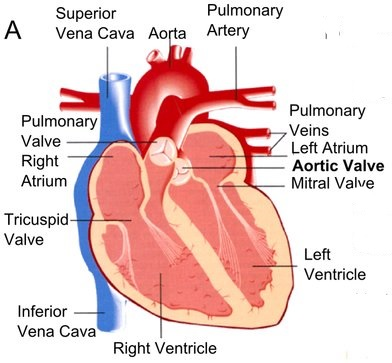
\includegraphics[width=\linewidth]{figures/heartimage.jpg}
    \captionof{figure}{Heart Valve System ~\citeonly{rockComplexCollagenFiber2014}}
    \label{fig:heart_valves}
}

The functionality and integrity of heart valves are essential for cardiovascular health. Heart valves open and close with each heartbeat, totaling over 3 billion times in a lifetime. This continuous operation occurs under significant pressure and within flowing blood, a viscous fluid rich in minerals, proteins, lipids, and cells. When valves become defective, they critically affect heart performance, leading to valve diseases that necessitate surgical intervention in the absence of curative drug treatments. Currently, diseased valves are replaced with artificial devices designed to emulate the valves' mechanical functions and restore heart functionality. However, these artificial valves can fail due to design flaws, material imperfections, or biocompatibility issues, often requiring risky reoperations. ~\citeonly{simionescuArtificialHeartValves2006}

Biomedical engineering strives to enhance treatments for valvular diseases, potentially impacting millions worldwide. This interdisciplinary field combines efforts from medicine, biology, engineering, and mechanics to improve device biocompatibility and explore tissue-engineering approaches that could enable the complete regeneration of valve tissues. ~\citeonly{simionescuArtificialHeartValves2006}

% \mynewline
% In summary, the heart valve system is central to the efficient operation of the cardiovascular system, ensuring that blood flows correctly throughout the body. The ongoing challenge in biomedical engineering is to develop better treatments for valvular diseases, aiming to improve or replace the natural function of heart valves effectively.

\subsection{Anatomy of the tricuspid valve}
%     Detailed Anatomy of the \gls{TV}: Focus on the \gls{TV}, given your project's emphasis. Describe its location, structure (leaflets, annulus, chordae tendineae, papillary muscles), and how these components work together to ensure unidirectional blood flow.
The \gls{TV}, an integral component of the heart's valve system, is located between the right atrium and right ventricle. It plays a crucial role in ensuring unidirectional blood flow from the atrium to the ventricle, thus maintaining the efficiency of the cardiac cycle. The \gls{TV}'s anatomy is complex and consists of several key structures: the annulus, leaflets, chordae tendineae, and papillary muscles.
\marginpar{
    \centering
    \footnotesize
    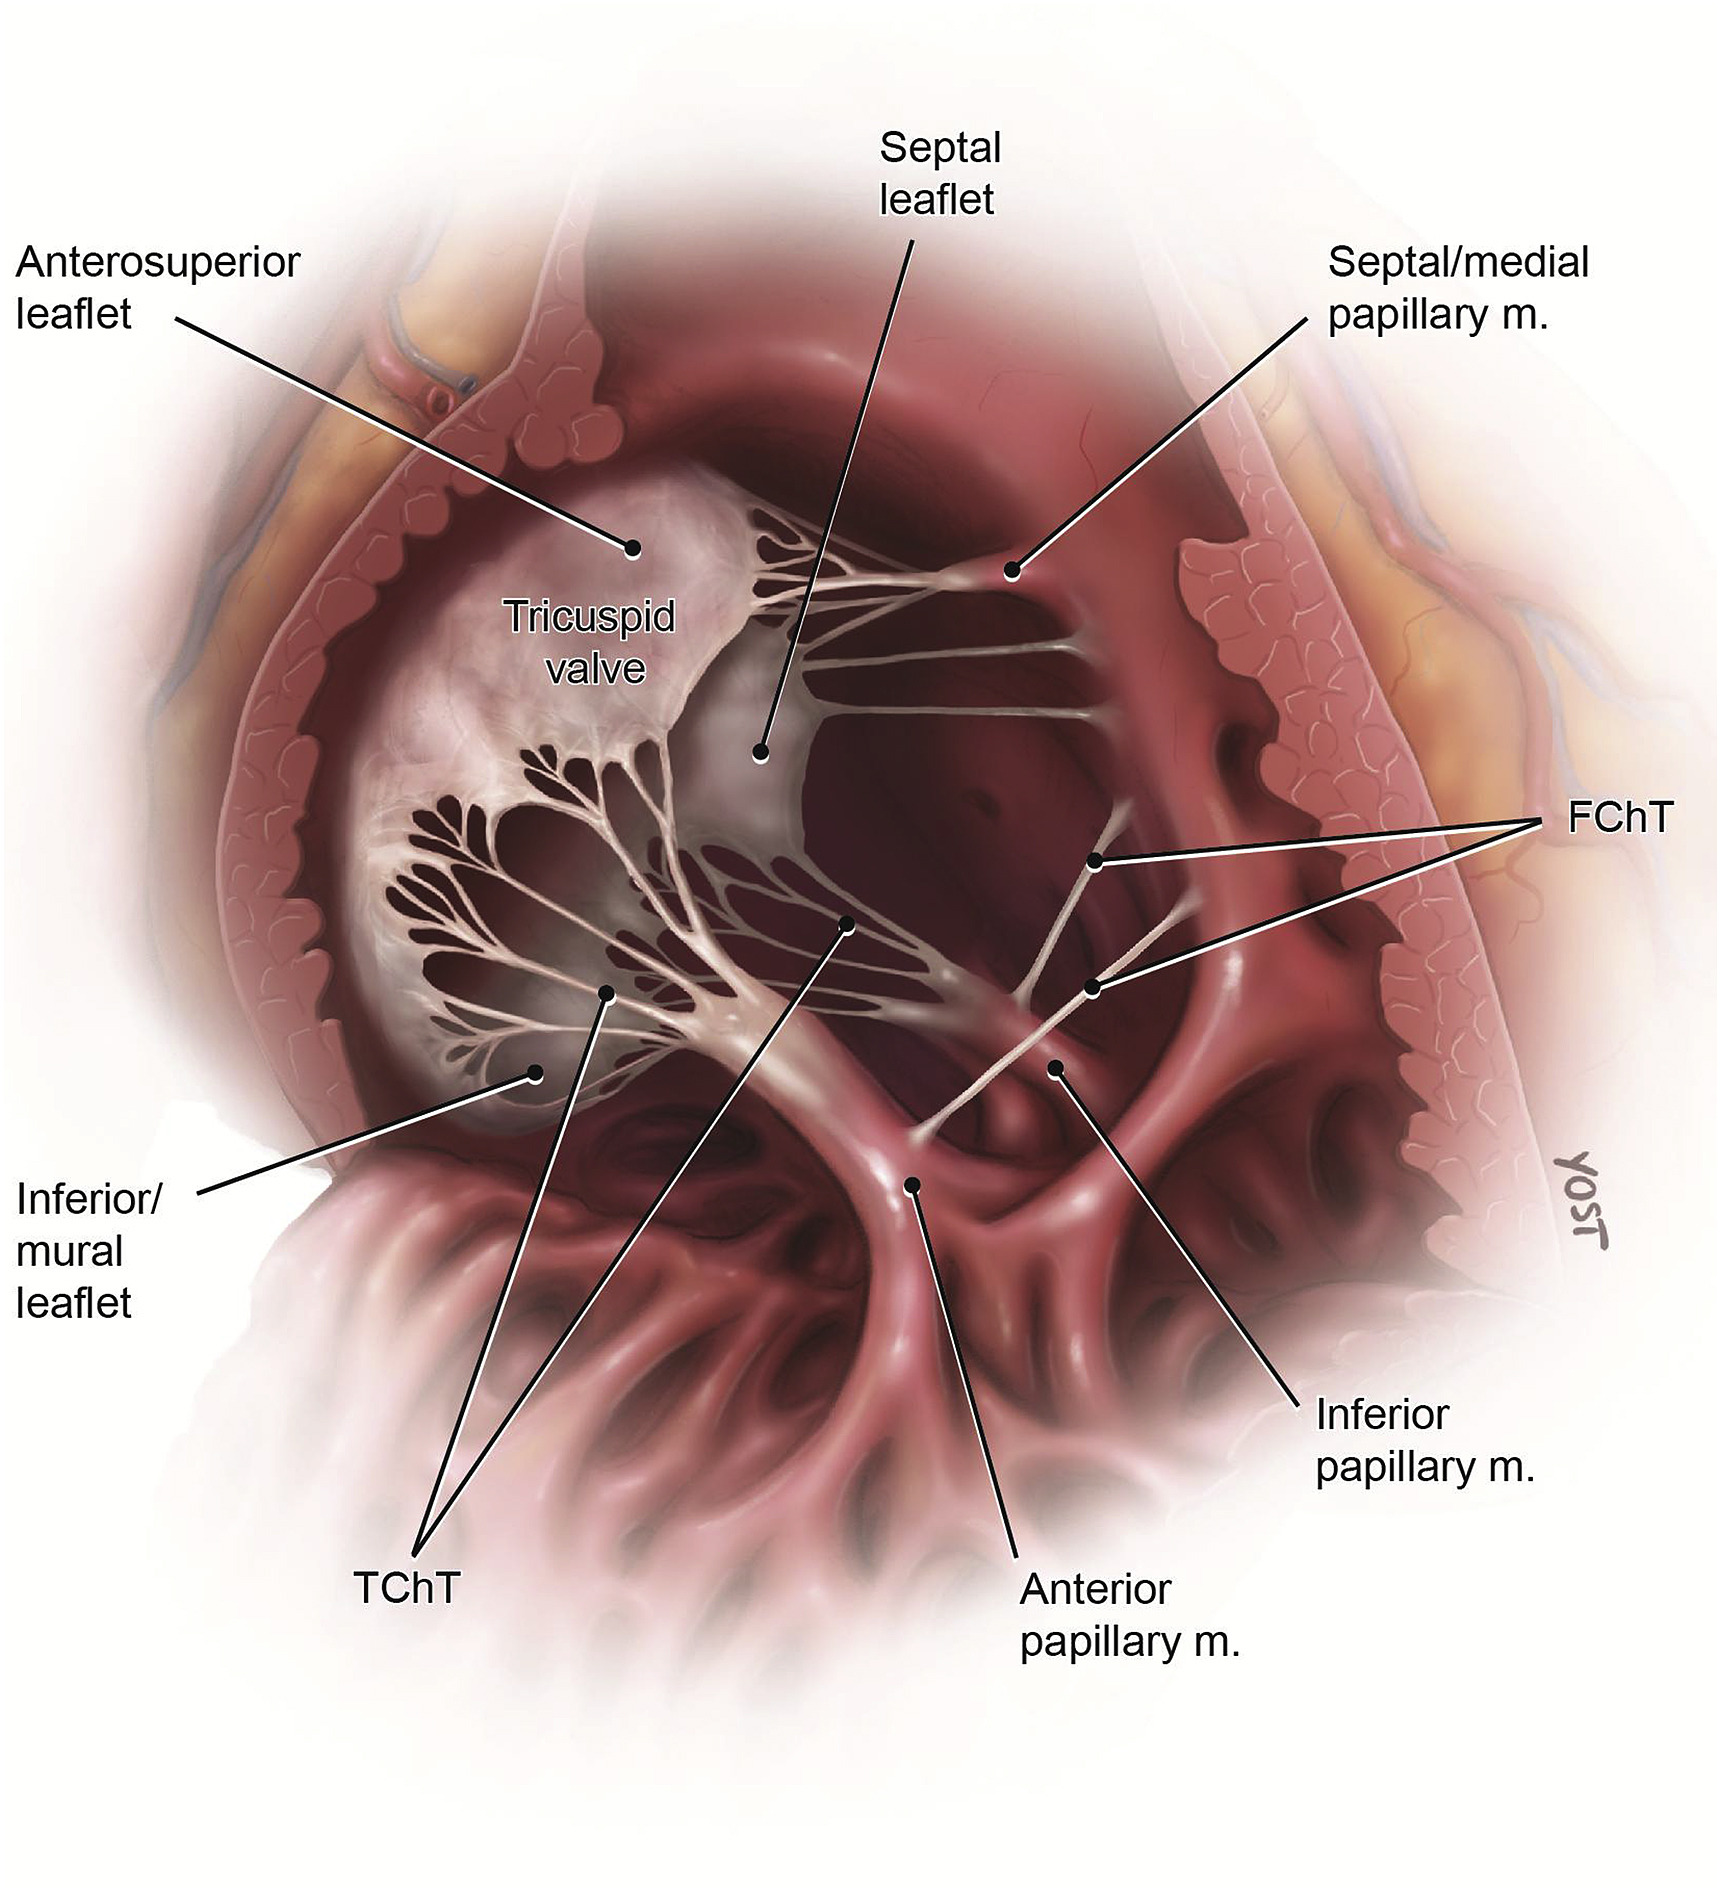
\includegraphics[width=\linewidth]{figures/tricuspidimage.jpg}
    \captionof{figure}{Sub-System of Tricuspid Valve ~\citeonly{YostDrawingDetailed}}
    \label{fig:tricuspid_valve}
}

\begin{itemize}
    \item Annulus: The annulus is a fibrous ring that anchors the valve leaflets and maintains their spatial configuration. It is the foundation to which the leaflets are attached, providing structural support for the entire valve apparatus.

    \item Leaflets: Typically, the \gls{TV} has three leaflets named according to their position: the anterior, posterior, and septal leaflets. These leaflets act as one-way doors that open to allow blood flow from the atrium to the ventricle and close to prevent backflow.

    \item Chordae Tendineae: These are thin, string-like structures that connect the valve leaflets to the papillary muscles. The chordae tendineae ensure the leaflets close securely and prevent them from inverting when the ventricle contracts.

    \item Papillary Muscles: These muscles extend from the inner walls of the right ventricle and attach to the valve leaflets via the chordae tendineae. During ventricular contraction, the papillary muscles contract, pulling the chordae tendineae taut and ensuring the valve leaflets close properly.
\end{itemize}

The \gls{TV}'s structure is characterized by its adaptability and variability. The number, length, and shape of the chordae tendineae and the papillary muscles can vary significantly among individuals, which can be of clinical significance. Dysfunctional papillary muscles or dysplastic chordae can lead to valve dysfunction, emphasizing the importance of understanding this complex anatomy for clinical assessment and intervention ~\citeonly{sandersTricuspidValveEmbryology2014}

Furthermore, the \gls{TV} is part of a dynamic apparatus that includes closely linked structures such as the annulus, leaflets, chordae, papillary muscles, and the right ventricle itself. Understanding the precise anatomy and function of these components is crucial for the success of percutaneous and surgical interventions aimed at addressing \gls{TV} pathologies ~\citeonly{buzzattiAnatomyTricuspidValve2018}
\subsection{Physiological Functioning}
%     Physiological Functioning: Explain the opening and closing mechanisms during the cardiac cycle, including the role of pressure changes in the heart chambers. Discuss the implications of valve malfunction (e.g., regurgitation, stenosis) on heart function.
The human heart contains four main valves: the mitral, tricuspid, aortic, and pulmonary valves. These valves play a critical role in ensuring unidirectional blood flow through the heart's four chambers, contributing to the efficiency of the cardiovascular system. The opening and closing of these valves are tightly regulated by pressure changes in the heart chambers during the cardiac cycle.

\newthought{Mechanism of Valve Functioning:}
\begin{itemize}
    \item During diastole, the mitral and \gls{TV}s open in response to pressure differences, allowing blood to flow from the atria to the ventricles.
    \item As the ventricles contract in systole, the mitral and \gls{TV}s close to prevent backflow of blood into the atria. Concurrently, the aortic and pulmonary valves open, allowing blood to be ejected from the ventricles to the aorta and pulmonary artery, respectively.
    \item When ventricular pressure falls below that in the aorta and pulmonary artery at the end of systole, the aortic and pulmonary valves close to prevent the backflow of blood into the ventricles.
\end{itemize}

\newthought{Implications of Valve Malfunction:}
\marginpar{
    \centering
    \footnotesize
    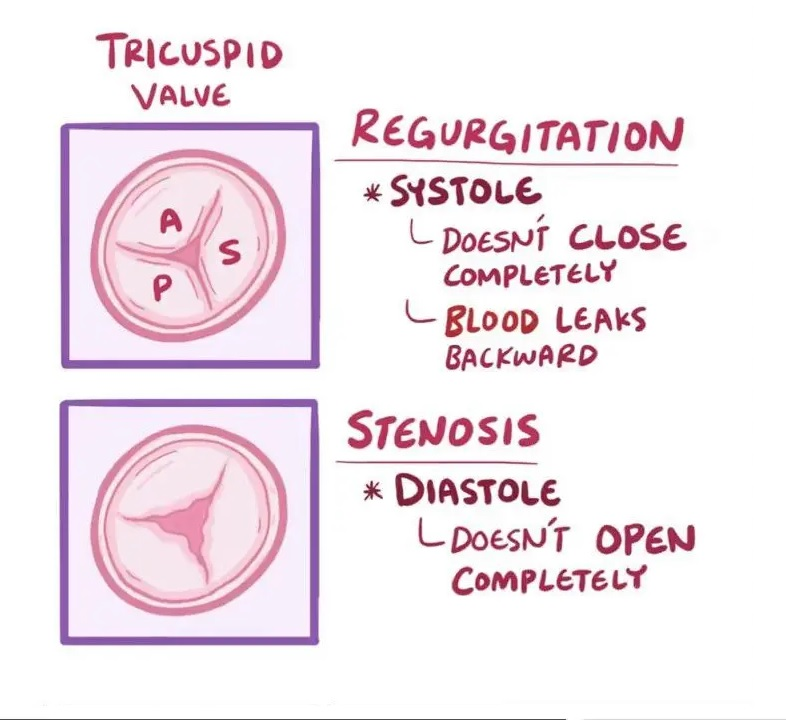
\includegraphics[width=\linewidth]{figures/regurgsteno.jpg}
    \captionof{figure}{Illustration of Regurgitation vs Stenosis ~\citeonly{TricuspidValveDisease}}
    \label{fig:regurg}
}
\begin{itemize}
    \item Valvular Stenosis: Stenosis of a valve leads to a narrowing of the valve opening, restricting blood flow. This results in increased workload for the heart chambers upstream of the affected valve, potentially causing hypertrophy and, ultimately, heart failure.
    \item Valvular Regurgitation: Valve regurgitation occurs when a valve does not close properly, allowing blood to flow backward. This leads to volume overload in the affected chambers, requiring the heart to work harder to pump the additional volume, which can also lead to heart failure over time.
\end{itemize}
Both conditions, if severe, can significantly impair cardiac function and may require surgical intervention, such as valve repair or replacement, to restore normal blood flow dynamics and prevent further cardiac damage. For instance, afterload mismatch in valvular heart disease, particularly in aortic stenosis, occurs when the left ventricle is unable to generate sufficient pressure to overcome the increased afterload caused by the stenosed valve, leading to a decrease in cardiac output. Surgical therapy, like aortic valve replacement, can relieve this mismatch and improve cardiac function, underscoring the importance of timely intervention in patients with valvular heart disease ~\citeonly{rossAfterloadMismatchAortic1985}.
\todo{maybe delete}


%     Variability and Pathologies: Briefly touch on common variations in \gls{TV} anatomy and how they might affect valve function. Also, review pathologies that can affect the valve, underscoring the need for effective simulation models.
\subsection{Variability and Pathologies}\label{sec:varpath}
The \gls{TV} is an essential component of the heart's right side and plays a critical role in the unidirectional blood flow from the right atrium to the right ventricle. Its anatomy and functioning can be affected by various factors, highlighting the importance of understanding its variability and pathologies;

\newthought{Anatomical Variability:}\\
The \gls{TV} typically features three leaflets (anterior, septal, and posterior), supported by chordae tendineae and papillary muscles. However, there can be considerable anatomical variability, including the number and size of leaflets, the structure of the subvalvular apparatus(papillary muscles, chordae tendineae and free wall), and the annular size. Such variations can impact valve function and are crucial for distinguishing between normal anatomical diversity and pathological alterations. In some instances, additional leaflets or unusual leaflet sizes are observed, affecting the valve's competence and flow dynamics. Understanding these variations is essential for accurate diagnosis and treatment planning, especially in surgical repairs and replacements .~\citeonly{tretterAssessmentAnatomicalVariation2016}

\newthought{Pathologies Affecting Valve Function:}\\
\gls{TV} pathologies can be classified into primary, involving intrinsic valve anatomy alterations, and secondary, resulting from functional modifications due to other cardiac or systemic conditions.
\begin{itemize}
    \item Primary \gls{TV} disease encompasses congenital abnormalities, infective endocarditis, rheumatic disease, and degenerative changes.
    \item Secondary \gls{TV} disease is often related to left heart diseases or pulmonary hypertension, leading to tricuspid annular dilation and right ventricular remodeling. These changes can result in tricuspid regurgitation or, less commonly, tricuspid stenosis, significantly impacting cardiac function and patient prognosis.
\end{itemize}
Advanced imaging techniques are crucial for the detailed evaluation of \gls{TV} anatomy and pathology, aiding in the accurate assessment and management of these conditions.~\citeonly{shahTricuspidValveDisease2008} One key aspect of tricuspid regurgitation that this study is looking to capture is the remodelling affects that tricuspid regurgitation has on the right ventricle and the valvular apparatus, some key variables that changes are the annular dilation, annular height, and circularity, which have been shown to increase in \citeonly{namModelingTricuspidValve2023} and chordal/papillary muscle lengths in \citeonly{obaseElongationChordaeTendineae2016}. All of these parameters are hoped to be captured over the study.

\newthought{Need for Effective Simulation Models:}\\
Given the complex anatomy of the \gls{TV} and the wide range of pathologies that can affect it, there is a growing need for effective simulation models. These models, computational and experimental can help in understanding the functional impacts of anatomical variability and pathological changes on the \gls{TV}, facilitating the development of more precise diagnostic tools and treatment strategies. Such models are particularly valuable in planning surgical interventions and predicting their outcomes.

\section{Advances in Heart Valve Disease Treatment}
%     Treatment Innovations: Review current and emerging treatments for \gls{TV} disease, including surgical interventions, transcatheter valve repair, and replacement therapies. Highlight how advancements in valve modeling and simulation could impact treatment outcomes or the development of new therapeutic techniques.
The landscape of treatments for \gls{TV} disease has been evolving, incorporating both surgical interventions and transcatheter approaches to offer alternatives for patients with varied risk profiles. Surgery remains the standard treatment for \gls{TV} disease, with techniques such as annuloplasty, leaflet repair, or valve replacement being common. However, surgical intervention is often reserved for patients without significant comorbidities due to the invasive nature of the procedures and the associated recovery times.

\newthought{Transcatheter Developments:}\\
Transcatheter techniques have emerged as a forefront innovation for treating \gls{TV} disease, especially for high-risk patients for whom traditional surgery is not viable. Transcatheter \gls{TV} repair and replacement therapies have shown promise in reducing tricuspid regurgitation and improving patient outcomes with less invasiveness than traditional surgery.
\begin{itemize}
    \item In transcatheter tricuspid valve repair various devices and techniques are being developed and tested, including coaptation devices, annuloplasty systems, and heterotopic caval valve implantation. These approaches aim to reduce tricuspid regurgitation by improving leaflet coaptation or reducing annular dilatation, offering symptomatic relief and functional improvement to patients with severe tricuspid regurgitation. ~\citeonly{hellComputedTomographyImaging2021}

    \item Transcatheter tricuspid valve replacement involves the percutaneous placement of a new valve within the native tricuspid annulus or a previously implanted surgical valve. This method has been advantageous for patients with severe \gls{TV} disease who are ineligible for surgical repair or replacement, demonstrating comparable safety and short-term outcomes. ~\citeonly{galesTranscatheterValveReplacement2018}
\end{itemize}
\begin{figure}[H]
    \centering
    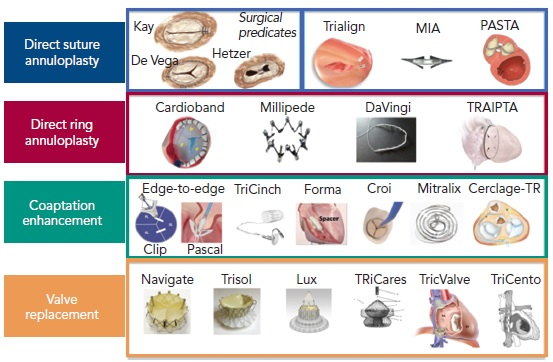
\includegraphics[width=\linewidth]{figures/TTVR.jpg}
    \caption{Current landscape of \gls{TTVR} products being used surgically ~\citeonly{curioUpdateCurrentLandscape2019}}
    \label{fig:TTVR}
\end{figure}

\newthought{Impact of Valve Modelling and Simulation:}\\
Advancements in valve modeling and simulation have significantly impacted the development of new therapeutic techniques for \gls{TV} disease. High-fidelity models created from patient-specific anatomical data have been instrumental in the design and testing of transcatheter devices, allowing for the precise customization of treatments. Computational simulations have also been crucial in understanding the biomechanical properties of the \gls{TV} under various physiological conditions, aiding in the optimization of device designs for improved durability and performance. These innovations in modelling and simulation hold the potential to enhance treatment outcomes for \gls{TV} disease, paving the way for the development of more effective and less invasive therapeutic options.

\section{Current Models and Simulators}

\subsection{Early Developments and Evolutation of Physcial Simulators}
The development of simulators in the field of cardiac care has a rich history, tracing back to the mid-20th century when the first conceptual models of blood flow dynamics and heart mechanics were introduced. These early models were primarily analog systems that used electrical circuits to mimic the hydraulic and hemodynamic properties of the heart. A pivotal innovation during this period was the development of the Windkessel model ~\citeonly{westerhofArterialWindkessel2009}, which was crucial in understanding arterial load and its effects on cardiac function, it described the haemodynamics of the arterial system in terms of resistance and compliance. It explained aortic pressure decay in diastole, but fell short in systole.
\marginpar{
    \centering
    \footnotesize
    \includegraphics[width=\linewidth]{figures/WindKessel.jpg}
    \captionof{figure}{Concept of the WindKessel Model ~\citeonly{westerhofArterialWindkessel2009}}
    \label{fig:wk}
}
The development of physical simulators has come hand in hand with clinical, computational and biological research advancements. Increases in computational power have allowed for the development of more advanced finite element models of the heart, which can simulate complex interactions between blood flow and heart valve mechanics. Software advancements have also played a critical role, with tools capable of simulating \gls{FSI} in the heart. Tangental clinical and biological studies have given more reason to develop physical simulators as now new hypotheses can be drawn from their learnings and then tested in a physical model.

The advent of 3D printing and \gls{CAD} technologies has revolutionized the fabrication of physical heart valve simulators. These technologies allow for high precision and customization of simulator components, enabling the production of complex valve geometries that accurately represent diverse anatomical variations seen in the population. This capability is vital for developing simulators that can be used for specialized surgical training and pre-surgical planning.

\subsection{Current State of the Art Simulators}

Heart valve models and simulators have significantly advanced, providing diverse tools for educational purposes, surgical planning, and research. These models range from low-fidelity simulators for basic educational use to high-fidelity, patient-specific models for complex surgical planning and research on prosthetics or interventions.

\newthought{Surgical Planning and Educational Models:}\\
Low-fidelity models, often made from commonly available materials, are used primarily for educational purposes. They provide an accessible and cost-effective means for trainees to develop surgical skills and understand valve anatomy and function. For instance, novel simulators made from components like baby bottles, combined with dental dam, offer simulation training in mitral and \gls{TV} surgical techniques, almost anywhere, at minimal cost. These models have been evaluated positively for their ability to replicate anatomy and surgical handling, proving very useful as training tools for cardiac surgery ~\citeonly{verberkmoesNovelLowfidelitySimulator2013}\\

One attempt at such an educational simulator took an entirely tissue-based approach. ~\citeonly{ramphalHighFidelityTissuebased2005} This offered a realistic environment for training cardiac surgical residents, replicating a variety of cardiac surgical procedures. They are instrumental in low-volume cardiothoracic surgery units, providing trainees with pre-clinical experience and helping them respond to clinical situations associated with heart-lung bypass machine operation and changes in patient clinical parameters.\\

Advanced, high-fidelity models are developed for surgical planning and research, employing technologies like 3D printing and silicone casting to create patient-specific valve models. These models enable simulation under dynamic physiologic conditions, allowing for the testing of surgical repairs and interventions with considerable accuracy. For example, dynamic ventricular simulators, capable of testing the quality of simulated heart valve procedures, utilize 3D printed valve suspension chambers and model pulsatile pumps to provide close-to-physiologic hemodynamic conditions for education and training in cardiac surgery ~\citeonly{zilinskasPhysiologicalVentricularSimulator2022}\\

Simulation models for valve surgery, like those for mitral valve repair, offer detailed physiological simulation, including real-time feedback mechanisms. These models incorporate integrated sensors to generate, record, and display quantitative data on trainee performance, significantly enhancing the learning experience ~\citeonly{tozziHeartSurgerySimulator2022}\\

Utilizing 3D printed valve suspension chambers and model pulsatile pumps, these simulators offer close to physiologic hemodynamic conditions. They have been validated for testing aortic valve leaflet repairs and replacements, demonstrating the potential for extensive educational use in cardiac surgery. ~\citeonly{zilinskasPhysiologicalVentricularSimulator2022}\\

Computational models are developed based on patient-specific data to predict clinical outcomes, aiding in planning medical procedures such as percutaneous pulmonary valve implantation and surgical repair of congenital heart diseases. These simulations have shown good agreement with clinical decisions, demonstrating their utility in personalized cardiovascular treatments. ~\citeonly{capelliPatientspecificSimulationsPlanning2017}

\newthought{Research-focused Models:}\\
For research, especially in developing prosthetics and testing interventions, simulators that can replicate the heart's mechanical and hemodynamic environment under various conditions are utilized. These include both native heart valve simulations and artificial heart valve simulations, categorized based on the prototype model. Such models are pivotal in studying valve biomechanics, facilitating predictive surgical planning, and aiding in the design and evaluation of repair devices and prostheses ~\citeonly{zhongNumericalSimulationDynamics2014}\\

Simulators designed to house an entire explanted heart subjected to pulsatile fluid-dynamic conditions enable the hemodynamic analysis of simulated surgical procedures. These setups are beneficial for device testing, offering a platform for in-depth investigation of valvular surgeries and interventions. ~\citeonly{leopaldiVitroHemodynamicsValve2012}


\newthought{Fidelity to Human Anatomy and Physiology in  Simulators:}\\
\begin{itemize}
    \item Some \gls{BHV}'s, such as the Texas TriValve 1.0, have made significant strides in computationally capturing the kinematics and kinetics of the native \gls{TV}. This model, reverse-engineered from a beating human heart, showcases how finite-element models can closely mimic the natural function of the \gls{TV}, including disease-induced and repair-induced changes. This level of detail offers a promising platform for simulating surgical and transcatheter interventions, aiming to improve patient outcomes. ~\citeonly{mathurTexasTriValveReverseengineered2022}
    \item Advanced simulators and models, especially those using 3D printing and computational simulations, have demonstrated a high degree of anatomical and physiological accuracy. These models can replicate complex heart valve geometries and dynamics, providing realistic conditions for training, surgical planning, and device testing. ~\citeonly{rabbahNovelLeftHeart2013}

    \item Anatomical and Mechanical Studies: Comparative studies have been crucial in understanding the mechanical, morphological, and microstructural differences between the mitral and tricuspid leaflets and chordae tendineae. These studies reveal that while there are no major differences in leaflet mechanics between the two valves, chordal mechanics can vary significantly, influenced by anatomical location and valve type. This information is vital for surgical and computational applications, especially considering the \gls{TV}'s unique stresses and strains. ~\citeonly{pokutta-paskalevaComparativeMechanicalMorphological2019}
\end{itemize}

\newthought{Paper released March 2024 - post thesis work conducted}
\begin{itemize}
    \item A research group in Heidelberg ~\citeonly{karlExvivoInvitroDynamic2024} developed a rig for mitral valve investigations in a manner similar to the aims of this project as they worked to investigate the effects of the MitraClip device. The rig was designed with less anatomical accuracy and not allowing \gls{PIV} measurement however this allowed the group to implement fixturing for motorized chordae tendineae adjustment and a camera system very close up and head-on to the valve to capture the coaptation process.
          \marginpar{
              \centering
              \footnotesize
              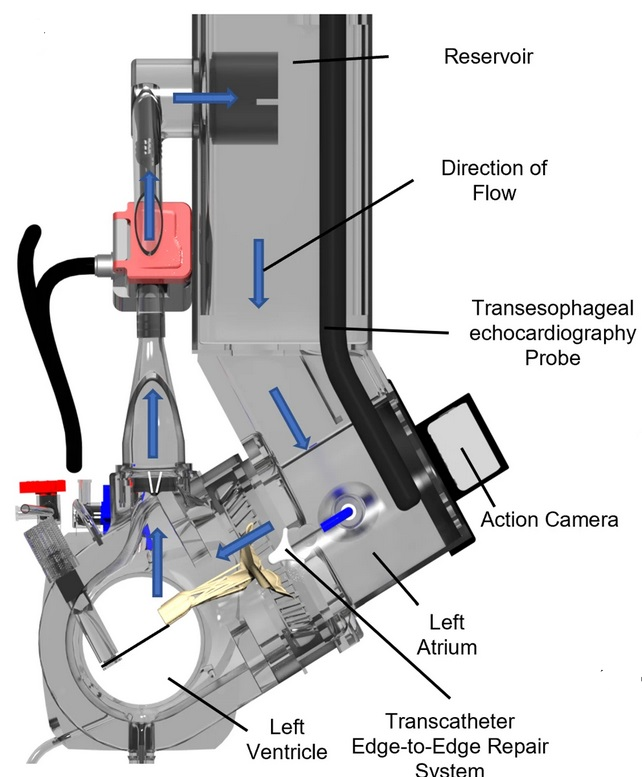
\includegraphics[width=\linewidth]{figures/karl2.jpg}
              \captionof{figure}{Side cross section of simulator with dynamic statecamera attachment ~\citeonly{karlExvivoInvitroDynamic2024}}
              \label{fig:k1}
          }
          \marginpar{
              \centering
              \footnotesize
              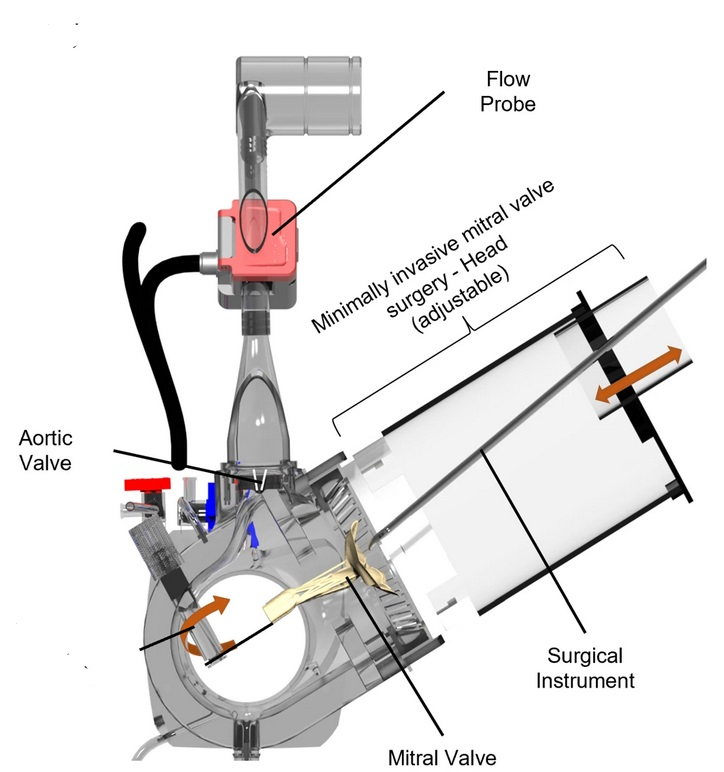
\includegraphics[width=\linewidth]{figures/karl1.jpg}
              \captionof{figure}{Side cross-section with static state surgery attachment ~\citeonly{karlExvivoInvitroDynamic2024}}
              \label{fig:k2}
          }
          This study ran a few different experiments, one with a mitral valve prosethesis, one with a mechanical valve, two with ex-vivo valves that were sewn onto an oversized elliptical frame and one experiment most close to the nature of this thesis where an in-vitro valve was
\end{itemize}
\newthought{Impact on Understanding Valve Mechanics and Patient Outcomes:}\\
Simulators play a crucial role in understanding the intricate mechanics of heart valves under various physiological and pathological conditions. They provide a risk-free environment for exploring new surgical techniques and device interventions, which is critical for advancing cardiac care. By allowing for the simulation of complex cardiac procedures and the testing of prosthetic valves and annuloplasty rings, these tools help improve surgical precision and patient outcomes. The feedback and data generated from simulators enable continuous learning and adaptation of best practices in heart valve surgery and intervention.

\section{Materials and Methods in Valve Modeling}

\subsection{Materials Used in Valve Modeling}
The development of heart valve models utilizes a range of materials, from biological tissues to synthetic polymers. These materials are selected based on their ability to simulate the natural behavior of heart valves, which is critical for ensuring the models' effectiveness in clinical training, pre-surgical planning, and device testing.
\marginpar{
    \centering
    \footnotesize
    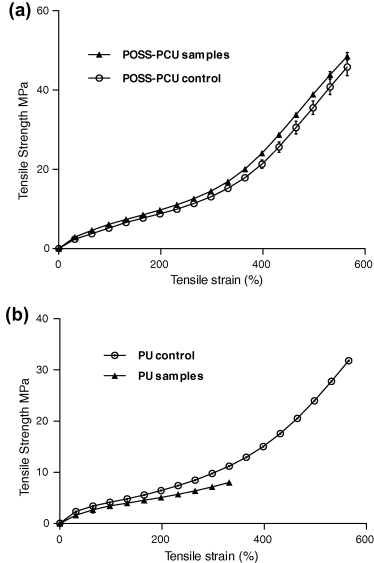
\includegraphics[width=\linewidth]{figures/PUanal.jpg}
    \captionof{figure}{Comparison of \gls{PU} and poly(carbonate-urea)urethane for heart valve performance ~\citeonly{ghanbariAnticalcificationPotentialSilsesquioxane2010}}
    \label{fig:punanal}
}
\newthought{Biological Tissues:}\\
Biological tissues have been a cornerstone in heart valve modeling, particularly for \gls{BHV} constructs. These tissues, typically derived from porcine or bovine sources, undergo treatments to enhance durability and reduce immunogenicity. The inherent biological properties of these tissues, such as their biomechanical behavior and hemocompatibility, make them suitable for simulating natural heart valve function. Limitations such as potential calcification, immune reactions have been shown however porcine and bovinepericaridium remains commonplace in current \gls{TTVR} and \gls{TAVR} respectively. ~\citeonly{filovaTissueengineeredHeartValves2009}

\newthought{Emerging Materials and Technologies:}\\
Recent advancements have led to the exploration of nanocomposite polymers \sidenote{essentially adding nano-sized building blocks into the polymer matrix which enhances durability while maintaining flexibility and processability} and hydrogels for heart valve modeling. Nanocomposite polymers, such as poly(carbonate-urea)urethane integrated with polyhedral oligomeric silsesquioxanes, exhibit enhanced mechanical properties and biostability. These materials show reduced calcification potential under in vitro conditions, making them attractive for the development of synthetic leaflet heart valves ~\citeonly{ghanbariAnticalcificationPotentialSilsesquioxane2010}

Hydrogels, derived from natural or synthetic sources, are being investigated for their potential in valve tissue engineering due to their biocompatibility and ability to support cell adhesion and proliferation. Challenges exist in balancing the bioactivity and mechanical durability of hydrogels to meet the demands of heart valve function.\citeonly{zhangApplicationHydrogelsHeart2015}

\marginpar{
    \centering
    \footnotesize
    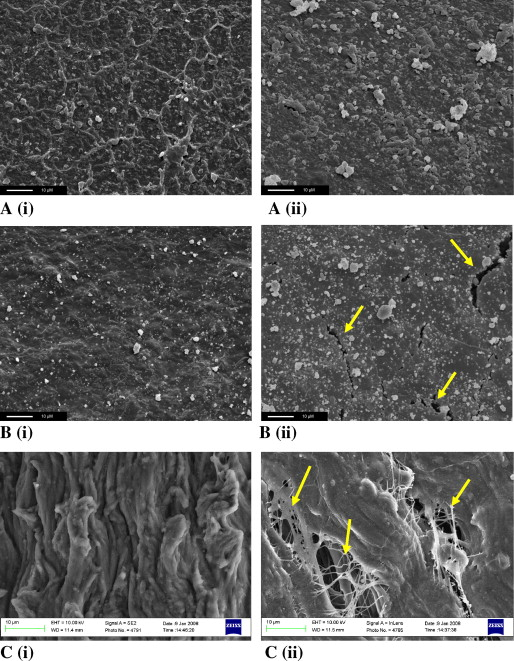
\includegraphics[width=\linewidth]{figures/PUanal2.jpg}
    \captionof{figure}{Comparison surfaces in fatigued (a) \gls{PU}  (b) poly(carbonate-urea)urethane (c) valve leaflets showing tissue failure  and fibre dehiscence marked by the yellow arrows in each ~\citeonly{ghanbariAnticalcificationPotentialSilsesquioxane2010}}
    \label{fig:puanal2}
}

\subsubsection{Synthetic Polymers:}
Synthetic polymers offer an alternative to biological tissues with advantages in consistency, durability, and the potential for customization. Polyurethane, silicone rubber, and \gls{PET} are among the polymers explored for heart valve modeling. Polyurethane, in particular, has shown promise due to its excellent tear resistance and similarity to the mechanical properties of natural valve tissue. The flexibility and durability of \gls{PU} make it an appealing choice for synthetic heart valve leaflets, though challenges remain in mimicking the viscoelastic properties of natural valves. ~\citeonly{baxterChapter12Selection2006} \sidenote{In the context of this project, choosing a synthetic material is desirable due to the intrinsic need of longevity so finding a \gls{PU} similar to those in valve replacements that can mimic the \gls{TV}'s function is}

\newthought{Silicone Mitral Valve Study}
The Engelhardt group \citeonly{engelhardtFlexibleComprehensivePatientspecific2019}
\begin{figure}[H]
    \centering
    \href{https://link.springer.com/article/10.1007/s11548-019-01971-9#MOESM1}{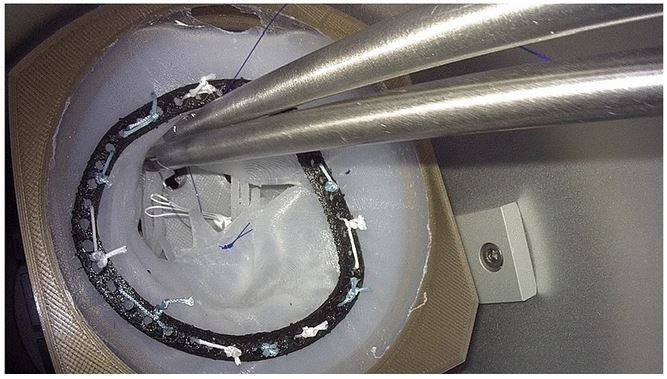
\includegraphics[width=\linewidth]{figures/Engel}}%
    \caption{Video of annuloplasty being performed on silicone mitral valve \textbf{(click to view video)}}
    \label{fig:Videoengel}
\end{figure}

\newthought{}
\citeonly{gintyModelingPatientSpecificDeformable2018}

\todo{finish this paper disc}
\newthought{Polyurethane Mitral Valve Study}
\citeonly{luoEffectBendingRigidity2012}
0.125mm average thickness, chordae 0.7mm diam, modelled in systole, leaflet youngs modulus 5.4mpa\ chordae youngs 30mpa

small Youngs modulus (~0.5 MPa) and high extensibility (~900\%) of the silicone alone. MV structures such as primary chordae tendineae have a higher Youngs modulus (~85 MPa) and a lower extensibility (4.3\%)\citeonly{liaoStructuralBasisSizerelated2003}



% \subsection{3D Printing and Fabrication Techniques}
%     3D Printing and Fabrication Techniques: Dive into modern fabrication techniques, especially 3D printing, used in valve model creation. Discuss the advantages of these methods in achieving anatomical precision and customizability.


\subsection{From Anatomical Data to Model}
%     From Anatomical Data to Model: Explain the process of translating anatomical data (e.g., from \gls{CT} scans, MRI) into functional models. Discuss the importance of accurate data and advanced imaging techniques in creating realistic models.
\newthought{Precedent of left heart valve models:}\\
In the process of translating anatomical data from \gls{CT} scans and \gls{MRI} into functional heart valve models, researchers have developed sophisticated methods to accurately capture the complex geometry and dynamics of the heart's valvular apparatus. This transition from imaging data to practical, patient-specific models is pivotal in advancing cardiac care, offering insights for surgical planning, device testing, and personalized treatment strategies.

~\citeonly{ionasecPatientSpecificModelingQuantification2010} introduced one of the first automatic computational systems for patient-specific modeling and quantification of the left heart valves, operating on cardiac \gls{CT} and transesophageal echocardiogram data. Their method, leverages discriminative learning and estimates  parameters from volumetric slices, enabling a holistic representation of the aortic and mitral valves that accounts for anatomical variations.

In a similar vein, ~\citeonly{grbicCompleteValvularHeart2012} proposed a patient-specific model of cardiac valves from 4D cardiac \gls{CT} data. Their model addresses the anatomical, functional, and hemodynamic aspects of the heart, utilizing a constrained Multi-linear Shape Model conditioned by anatomical measurements. This approach offers a more detailed representation of the heart's valvular structures and dynamics, facilitating the study of valvular pathologies and interventions.

\todo{Finish this paper disc}
One research group has done multiple studies on making anatomical models for procedure planning and device testing. The group 3d printed semi flexible material to implant the MitraClip device\citeonly{vukicevic3DPrintedModeling2017} and later did the same for the tricuspid valve \citeonly{vukicevicPatientSpecific3DimensionalPrinted2020}

\newthought{Challenges with Right Heart:}\\
The challenges of the right heart stem primarily from the complex anatomical and functional nature of the \gls{TV}, which can be more difficult to capture accurately due to several factors:

\begin{itemize}
    \item The \gls{TV}'s structure includes multiple leaflets (usually three) and a complex subvalvular apparatus, which are not symmetrically arranged. This complexity makes it harder to capture and model accurately using standard imaging techniques compared to the more symmetrically structured mitral valve.

    \item Both CT and MRI rely on good contrast resolution to differentiate between structures. The right heart's lower pressure and flow conditions can result in poorer contrast enhancement of the \gls{TV}, further complicating accurate imaging and subsequent modeling.~\citeonly{ahnTricuspidValveImaging2021}

    \item The tricuspid valve is subject to significant motion during the cardiac cycle, and capturing its dynamic behavior accurately with CT and MRI is challenging due to potential motion artifacts.~\citeonly{suhWholeheartMotioncorrectionAlgorithm2017}
\end{itemize}

\mynewline
While these challenges have slowed progress, research on the right-heart is catching up and with techniques like \gls{CT} motion-correction algorithms and wide-detector \gls{CT} with low radiation doses ~\citeonly{ahnTricuspidValveImaging2021, suhWholeheartMotioncorrectionAlgorithm2017} so the benefits of patient specific modeling can be extended to the right heart as well.


\subsection{Evaluation and Testing Methods}
%     Evaluation and Testing Methods: Conclude by discussing how valve models are evaluated and tested for their functionality. Include methodologies for assessing their mechanical properties, durability, and physiological accuracy in simulating heart valve dynamics.
The evaluation and testing of heart valve models are crucial to ensure their functionality, mechanical properties, durability, and physiological accuracy. Several methodologies have been developed to assess these aspects, employing both in vitro and computational simulation techniques.

\newthought{Mechanical Properties and Durability Testing:}
\begin{itemize}
    \item Bench Testing to ISO Standards: ~\citeonly{stasiakDesignDevelopmentTesting2020} reported on the design, development, and testing of a polymeric heart valve, including bench testing according to ISO 5840:2015 standards. Their study highlights the importance of rigorous bench testing in evaluating valve hydrodynamics, durability (tested to over 1.2 billion cycles), and preliminary biocompatibility in short-term animal models. This comprehensive approach ensures that new valve designs meet international safety and performance standards before clinical application.
          \marginpar{%
              \footnotesize
              \textbf{Resources:}\\
              \begin{itemize}
                  \item \href{https://www.iso.org/obp/ui/en/\#iso:std:iso:5840:-1:ed-2:v1:en}{Revised ISO Overview}
              \end{itemize}
          }
    \item In Vitro Testing: ~\citeonly{walkerVitroEvaluationMechanical2010} developed a novel test chamber for an automated mock circulatory loop to evaluate the mechanical performance of heart valves. This method allows for the simulation of physiological flow conditions to assess valve functionality, durability, and potential thrombotic and hemolytic effects. Such setups are vital for understanding how artificial heart valves would perform under real-life conditions.
    \item ~\citeonly{thomasComputationalMultiscaleApproach2019} implemented a multiscale modeling approach to predict extracellular matrix microstructural changes in response to tissue-level mechanical stimuli in the \gls{TV}'s anterior leaflet. This study highlighted the importance of understanding microstructural alterations under mechanical loading for developing new tissue-engineered replacements.
\end{itemize}

\newthought{Physiological Accuracy and \gls{FSI} Models:}
\begin{itemize}
    \item  ~\citeonly{leeFluidStructureInteractionModels2020} developed dynamic computer models of \gls{BHV}s in an experimental pulse duplicator, based on the immersed boundary method for \gls{FSI}. These models simulate porcine tissue and bovine pericardial BHVs under conditions used to assess performance in commercial and custom pulse duplicators. The agreement between computational simulations and experimental data for bulk flow rates, pressures, and valve opening areas underscores the potential of \gls{FSI} modeling in valve design and evaluation.
    \item  ~\citeonly{damoreHeartValveScaffold2018} introduced double component deposition, an electrodeposition technique for fabricating valve scaffolds with controlled macro-scale morphology, mechanics, and micro-structure. This method allows for the creation of fully assembled stent-less multi-leaflet valves, demonstrating the capability of emerging fabrication techniques in producing scaffolds that closely mimic natural valve behavior.
    \item ~\citeonly{laurenceInvestigationRegionalVariations2019} conducted an investigation into the regional variations in the biaxial mechanical properties and stress relaxation behaviors of porcine atrioventricular heart valve leaflets. Their findings underscored the significance of accounting for regional differences in valve biomechanics to refine computational models for predicting diseased or surgically altered valve function. This approach allows for a more accurate simulation of heart valve dynamics and mechanical behavior under varying physiological conditions.
\end{itemize}







% Materials and Methods in Valve Modeling
%     Materials Used in Valve Modeling: Review the variety of materials used in constructing heart valve models, from biological tissues to synthetic polymers. Discuss the properties that make certain materials more suitable for simulating the natural behavior of heart valves.

\section{Regulatory and Ethical Considerations}

\subsection{Regulatory Standards for Valve Models and Simulators}
%     Regulatory Standards for Valve Models and Simulators: Discuss the regulatory environment surrounding the development and use of heart valve models and simulators, especially those intended for clinical training or pre-surgical planning. This may include standards for accuracy, safety, and efficacy.
The development and use of heart valve models and simulators, particularly those intended for biomedical engineering or pre-surgical planning, are governed by a comprehensive regulatory environment. This framework ensures that these tools meet stringent standards for accuracy, safety, and efficacy before being implemented in clinical settings.

\newthought{Experimental Validation and ISO Standards:}\\
The experimental validation of cardiac simulators, as described by ~\citeonly{bazanExperimentalValidationCardiac2016}, is a critical step in developing prosthetic heart valves. Their work underscores the importance of adhering to physiological conditions and meeting the requirements of ISO 5840 standards, which set global benchmarks for cardiovascular implants and cardiac valve prostheses. This ensures that simulators provide a suitable environment for testing valve performance in the mitral, aortic and tricuspid positions under varying heart rates.

% \newthought{Animal Models for Regulatory Compliance:}\\
% Preclinical testing in appropriate animal models is mandated by regulatory bodies like the Food and Drug Administration before human clinical trials. This in vivo testing, performed under strict regulatory guidelines, is essential for assessing the performance, durability, and biocompatibility of novel heart valve therapies. The careful selection of animal models and adherence to guidelines ensure the collection of relevant data while minimizing potential distress or discomfort to the test subjects, facilitating the transition from preclinical to clinical studies. ~\citeonly{ahlbergAnimalModelsCardiac2013}
\newthought{Safety Regulations:}\\
While physical simulators are not used within patients, they must still adhere to safety regulations to ensure they pose no hazard during use. This includes mechanical, chemical and electrical safety standards, especially for those simulators that involve interactive components or electronic devices. Regulators might require that these devices be certified safe for use in educational environments, involving regular maintenance and safety checks as well as proper training for users, personal protective equipment availability and general workplace safety.

\newthought{Living Heart Project and Integrative Simulators:}\\
The Living Heart Project represents a significant advancement in simulating human heart function through a four-chamber heart model. This integrative simulator showcases the potential of computational models of the whole heart, including its valves. Such initiatives illustrate how regulatory standards can evolve to include advanced computational methods and integrative simulators for heart valve research and development ~\citeonly{baillargeonLivingHeartProject2014} and how other research work can contribute to new regulatory standards and set a precedent for how future heart valve simulators should be conducted.

% \newthought{Considerations for Engineered Tissue Heart Valves:}\\
% The development pathway for tissue-engineered heart valves  presents unique regulatory challenges. ~\citeonly{zhangPreclinicalAssessmentCardiac2019} review the regulatory framework for medical devices and highlight the special considerations for tissue-engineered heart valves, emphasizing the importance of adhering to ISO 5840 guidelines and proposing a translational roadmap to navigate the complex regulatory environment. This underscores the necessity of a well-defined regulatory approach to ensure the safety and efficacy of emerging valve technologies.


\subsection{Ethical Implications}
%     Ethical Implications: Briefly touch on the ethical considerations in developing and deploying new heart valve treatments, with an emphasis on patient safety, informed consent, and access to innovation.
% The development and deployment of new heart valve treatments involve a complex interplay of ethical considerations. These considerations encompass ensuring patient safety, obtaining informed consent, and ensuring equitable access to innovations. Below are key points highlighting these ethical dimensions:
% \newthought{Patient Safety:}\\
% The paramount concern in the development of new heart valve treatments is patient safety. ~\citeonly{rajabChapterIIIEthical2013} delve into the ethical principles applied to biomedical research and development, emphasizing the necessity of prioritizing patient welfare throughout the development process of new prosthetic heart valves. Ensuring the safety of these innovations requires rigorous clinical trials and continuous monitoring for adverse effects post-implementation.
% \newthought{Informed Consent:}\\
% Obtaining informed consent is a critical ethical obligation when deploying new heart valve treatments. ~\citeonly{fletcherCardiacTransplantsArtificial1983} discusses the ethical framework within which medical decisions, including those relevant to cardiac transplantation and artificial hearts, are made, highlighting the importance of patient autonomy and informed decision-making. This involves ensuring that patients are fully aware of the potential risks and benefits of new treatments.
% \newthought{Access to Innovation:}\\
% Ensuring equitable access to innovative heart valve treatments is a significant ethical concern. ~\citeonly{aultmanEthicsRepeatHeart2018} examine the ethical issues surrounding repeat heart valve replacement surgery, particularly for patients with substance use disorders. This discussion extends to the broader issue of access to new and potentially life-saving treatments, irrespective of a patient's socio-economic status or other personal circumstances.
The development and deployment of physical heart valve simulators involve significant ethical considerations, especially concerning patient safety, informed consent, and access to innovative technologies.

\newthought{Patient Safety:}\\
The primary concern in the development of new heart valve simulators is to ensure patient safety. As these simulators are used in educational and pre-surgical planning, it is crucial that they accurately mimic human physiology to prevent potential errors during actual surgeries. Ensuring the safety and efficacy of these simulators involves rigorous testing and validation processes to avoid any adverse consequences during training sessions or surgical planning.~\citeonly{rajabChapterIIIEthical2013}

\newthought{Informed Consent:}\\
Although physical simulators are not implanted in patients, obtaining informed consent is crucial when they are used in scenarios that involve patient interaction, such as educational demonstrations or pre-surgical planning. Patients and participants should be fully informed about the procedures being simulated, the use of their data (if applicable), and the nature of the demonstrations to uphold ethical standards of autonomy and consent.~\citeonly{fletcherCardiacTransplantsArtificial1983}

\newthought{Access to Innovation:}\\
Access to high-quality educational tools and advanced simulators should be equitable to ensure that all medical professionals, regardless of their institution's economic status, have the opportunity to train with the best available tools. This is essential for maintaining high standards of healthcare globally and ensuring that advancements in medical training are accessible to all healthcare providers, thus broadening the benefits of innovative educational simulators.~\citeonly{aultmanEthicsRepeatHeart2018}

By addressing these ethical considerations, developers and users of heart valve simulators can ensure that their use in medical education and surgical planning is both effective and ethically sound, supporting the broader goals of improving patient care and surgical outcomes.

\section{Research Strengths and Gaps}

\subsection{Research Strengths}

\newthought{Advancements in Imaging and Computational Simulations:}\\
Recent years have witnessed significant advancements in imaging techniques and computational simulations, which have enhanced the understanding and modeling of heart valve mechanics. High-resolution imaging modalities such as 4D \gls{CT} and \gls{MRI} have enabled detailed anatomical and functional assessments of heart valves in real time. These advancements have facilitated the development of more accurate computational models that can predict how valves behave under various physiological and pathological conditions. Such models are invaluable for both pre-surgical planning and the design of prosthetic valves.

\newthought{Integration of Patient-Specific Data into Valve Design:}\\
The incorporation of patient-specific anatomical data into the design and testing of heart valves is a major strength in current research which can significantly enhance the efficacy and safety of treatments as outcomes can be predicted. This approach has led to the development of customized prosthetic valves as opposed to one-size-fits-all valves where there is increased risk of failure.~\citeonly{kidaneCurrentDevelopmentsFuture2009}

% \newthought{Development of Hybrid Models and Simulation Platforms:}\\
% Another key strength is the development of hybrid simulation models that combine both physical and computational elements. These hybrid platforms enable simultaneous analysis of mechanical and fluid dynamics aspects of valve operation, providing a comprehensive understanding of valve behavior under different conditions. Such models are crucial for the testing and verification of heart valve designs before they are used in clinical settings, ensuring that they meet the required performance standards.~\citeonly{yoganathanHybridApproachHeart2017}

\newthought{Regulatory and Standardization Advances:}\\
The establishment of standardized testing protocols and regulatory guidelines for heart valve devices is another significant strength. This regulatory framework supports innovation while ensuring patient safety and the reliability of heart valve products on the market. By adhering to these standards, researchers and manufacturers can develop and test heart valve devices more effectively.


\subsection{Research Gaps}

\newthought{Anatomical Variability:}\\
The significant anatomical variability of the \gls{TV} presents challenges in creating universally applicable models. For example, the presence of additional leaflets or variations in chordae tendineae and papillary muscles can significantly impact valve function and complicate the design of surgical interventions or prosthetic valves. Understanding and incorporating this variability into models remains a challenge.~\citeonly{tretterAssessmentAnatomicalVariation2016}

Being able to, with the same piece of equipment, account for changes like these in real-time would be greatly beneficial to studies on the \gls{TV} devices and interventions.

\newthought{Material Properties and Biomechanics:}\\
Accurately simulating the material properties and biomechanical behavior of the TV leaflets and subvalvular apparatus is complex. Finite element modeling studies have attempted to address this by adjusting material parameters and considering different collagen fiber distributions. However, these models still face limitations in accurately representing shear behavior and the complex interactions within the TV apparatus under various physiological and pathological conditions.~\citeonly{stevanellaFiniteElementModelling2010}

Developing materials that can mimic the viscoelastic properties of natural valve tissues and withstand the mechanical stresses of long-term operational testing is a critical gap in the field. This would afford researchers the time to gather more data on the same specimens in testing, increasing the reliability and statistical significance of the results.

\newthought{Dynamic Bench-Top Simulation Capabilities:}\\
Enhancing the dynamic response of simulators to replicate real-time cardiac motions and valve mechanics accurately. This includes the ability to simulate different heart rates, pressures, and pathological conditions to understand their impacts on valve function and durability as well as materials that accurately mimic the biomechanical properties of natural heart tissues, which is challenging due to the complex nature of biological tissues. These materials need to withstand the mechanical stresses of long-term operation to be effective for training and testing.

Current simulators have often opted for integrating disected porcine hearts into their setups rather than developing synthetic materials which can only withstand a very limited amount of testing before failure. This is a significant gap in the field as it limits the ability to perform long-term projects investigating aspects of valve design and function.
% \newthought{Weaknesses and Areas for Improvement:}

% \begin{itemize}
%     \item Material Properties and Biomechanics: Despite advancements, accurately simulating the material properties and biomechanical behavior of heart valves remains a challenge. There's a need for models that more accurately reflect the viscoelastic properties of valve tissues, which are critical for predicting long-term device performance and valve behavior under physiological conditions.
%     \item Dynamic Simulation Capabilities: Many models still struggle with simulating the dynamic interactions between blood flow and valve motion, especially under varying physiological conditions. Enhancing \gls{FSI} simulations would improve the realism of simulations and the predictive value of models for surgical and interventional planning.
%     \item Anatomical Variability: While patient-specific modeling has advanced, there's still a need to better account for the wide range of anatomical variability observed in heart valve structures among different individuals. Models and simulators must be adaptable to reflect this diversity accurately.
%     \item Long-term Durability and Failure Modes: Current simulators and models primarily focus on short-term functionality without adequately simulating long-term wear, material degradation, or failure modes of valves and valve replacements. Developing models that can simulate years of operation within a short time frame would be invaluable for predicting valve durability and identifying potential failure mechanisms.
% \end{itemize}

% \newthought{Innovations Needed:}
% \begin{itemize}
%     \item {Advanced Materials:}\\
%           Research into new materials that mimic the complex biomechanical properties of native valve tissues could improve the realism and predictive capability of valve models.
%     \item {Hybrid Simulation Approaches:}\\
%           Combining computational models with physical simulators could offer a more comprehensive approach to understanding valve mechanics and interventions, allowing for simultaneous assessment of anatomical, physiological, and biomechanical factors.
%     \item{Machine Learning and AI Integration:}\\
%           Leveraging machine learning algorithms to analyze outcomes from simulated valve interventions could identify patterns and predict outcomes, optimizing valve designs and surgical approaches.
%     \item{Enhanced \gls{FSI} Modeling:}\\Improving the fidelity of \gls{FSI} modeling would allow for more accurate simulations of blood flow dynamics and their impact on valve function, particularly under abnormal conditions.
% \end{itemize}


\begin{table}[H]
    \begin{fullwidth}
        \centering
        \footnotesize
        \noindent\makebox[\textwidth]{%
            % Please add the following required packages to your document preamble:
% \usepackage{multirow}

% \centering
% \begin{tabular}{p{50pt}|p{75pt}|p{75pt}|p{100pt}|p{50pt}|p{60pt}}
%     \hline
%     \textbf{Authors \& Year} & \textbf{Key Findings}                                                & \textbf{Study Objective}                                            & \textbf{Methodology}                                                                                & \textbf{Relevance to Your Study} & \textbf{Key Learnings}                        \\ \hline
%     Filová et al. 2009       & Calcification of PU in vivo                                          & Overview of tissue-engineered heart valves                          & Meta-Analysis                                                                                       & Material Choice                  & Limited sample size                           \\ \hline
%     Baxter et al. 2006       & Flexibility and durability of PU                                     & Overview of synthetic materials in heart valves                     & Tearing energy and crack growth rate tests                                                          & ~                                & Performs even better at elevated temperatures \\ \hline
%     Aggarwal et al. 2013     & Converting CT to 3D                                                  & To map patient-specific aortic valves                               & Spline-fitting with mathematic models using echocardiographic images                                & Modelling/Morphology             & Maps microstructure of leaflets               \\ \hline
%     Leopaldi et al. 2012     & Comparative data for experimental and simulatory flow-loop           & To develop a flow loop with a porcine heart                         & Endoscopic imaging and hemodynamic measured with ultrasound flowmeter and piezoelectric transducers & Simulator Development            & Compares pressures and flow rates             \\ \hline
%     Zilinskas et al. 2022    & Simulator succesfully used for performing valve replacement training & To develop a surgical training simulator using porcine aortic roots & Porcine aortic valve dissected and tether to chamber                                                & ~                                & Demonstrates efficacy of bench-top simulators \\ \hline
% \end{tabular}
% \label{littable}

\renewcommand{\arraystretch}{1.2}
\begin{tabular}{p{50pt}|p{75pt}|p{75pt}|p{110pt}|p{55pt}|p{75pt}}
  \textbf{Authors \& Year} & \textbf{Key Findings}                                                & \textbf{Study Objective}                                            & \textbf{Methodology}                                                                                & \textbf{Relevance to Your Study} & \textbf{Key Learnings}                        \\ \hline
  Filová et al. 2009       & Calcification of PU in vivo                                          & Overview of tissue-engineered heart valves                          & Meta-Analysis                                                                                       & Material Choice                  & Limited sample size                           \\
  Baxter et al. 2006       & Flexibility and durability of PU                                     & Overview of synthetic materials in heart valves                     & Tearing energy and crack growth rate tests                                                          & Material Choice                  & Performs even better at elevated temperatures \\
  Aggarwal et al. 2013     & Converting CT to 3D                                                  & To map patient-specific aortic valves                               & Spline-fitting with mathematic models using echocardiographic images                                & Modelling / Morphology           & Maps microstructure of leaflets               \\
  Leopaldi et al. 2012     & Comparative data for experimental and simulatory flow-loop           & To develop a flow loop with a porcine heart                         & Endoscopic imaging and hemodynamic measured with ultrasound flowmeter and piezoelectric transducers & Simulator Development            & Compares pressures and flow rates             \\
  Zilinskas et al. 2022    & Simulator succesfully used for performing valve replacement training & To develop a surgical training simulator using porcine aortic roots & Porcine aortic valve dissected and tether to chamber                                                & Simulator Development            & Demonstrates efficacy of bench-top simulators \\
\end{tabular}

% \centering
% \arrayrulecolor{black}
% \ADLnullwidehline
% \begin{tabular}{p{50pt}|p{75pt}|p{75pt}|p{100pt}|p{50pt}|p{60pt}}
%   \toprule
%   \textbf{Authors \& Year}                                                     & \textbf{Key Findings}                                                    & \textbf{Study Objective}         & \textbf{Methodology} & \multicolumn{1}{l!{\color{black}\vrule}}{\textbf{Relevance to Your Study}} & \textbf{Key Learnings} \\
%   \midrule
%   Filová et
%   al. 2009                                                                     & Calcification of PU in vivo                                              & Overview of tissue-engineered
%   heart valves                                                                 & \multicolumn{1}{l!{\color{black}\vrule}}{Meta-Analysis}                  & \multirow{2}{*}{Material Choice} & Limited sample size                                                                                                        \\
%   \cmidrule{1-4}\cmidrule{6-6}
%   Baxter et
%   al. 2006                                                                     & Flexibility and durability of PU                                         & Overview of synthetic materials
%   in heart valves                                                              & \multicolumn{1}{l!{\color{black}\vrule}}{Tearing energy and crack growth
%   rate tests}                                                                  &                                                                          & Performs even better at elevated
%   temperatures                                                                                                                                                                                                                                                                                                            \\
%   \midrule
%   ~Aggarwal et al. 2013                                                        & Converting CT to 3D                                                      & To map patient-specific aortic
%   valves                                                                       & Spline-fitting with mathematic
%   models using echocardiographic images                                        & Modelling / Morphology                                                   & Maps microstructure of leaflets                                                                                                                               \\
%   \midrule
%   Leopaldi
%   et al. 2012                                                                  & Comparative data for
%   experimental and simulatory flow-loop                                        & To develop a flow loop with a
%   porcine heart                                                                & Endoscopic imaging and
%   hemodynamic measured with ultrasound flowmeter and piezoelectric transducers & \multirow{2}{*}{Simulator Development}                                   & Compares pressures and flow
%   rates                                                                                                                                                                                                                                                                                                                   \\
%   \cmidrule{1-4}\cmidrule{6-6}
%   Zilinskas
%   et al. 2022                                                                  & Simulator succesfully used for
%   performing valve replacement training                                        & To develop a surgical training
%   simulator using porcine aortic roots                                         & Porcine aortic valve dissected
%   and tether to chamber                                                        &                                                                          & Demonstrates efficacy of
%   bench-top simulators                                                                                                                                                                                                                                                                                                    \\
%   \bottomrule
% \end{tabular}
% \arrayrulecolor{black}}
        \caption{Comparison of key points in the literature review}
    \end{fullwidth}
\end{table}

\begin{fullwidth}
  \part{Methodology}\label{pt:methodology}
\end{fullwidth}
\parttoc[n]
\chapter{Design and Prototyping}\label{ch:DesProt}
\vspace{-2.5em}
% \newthought{Synopsis}\synopsisChProcessing
\newthought{Synopsis}\synopsisDesign
\mynewline
\section{Conceptualisation and Initial Design}
The essence of a design process is inherently iterative and exploratory. It's a cyclical journey of conception, experimentation, evaluation, and refinement. This iterative cycle is fundamental to translating abstract ideas into tangible solutions that meet specific functional and operational goals.
%Within this framework, the development of a mock \gls{TV} for a heart simulator exemplifies the complex interplay of innovation, precision, and adaptability.

At the heart of the design process lies the concept of trial and error—a methodical yet flexible approach that takes the discovery of unexpected challenges and leverages them as opportunities for learning. Initial ideas are transformed into preliminary models, serving as the first step in a series of continuous interactions between designing, testing, and iterating.
%This process is characterized by the application of various modeling approaches, each iteration informed by the insights gained from previous attempts and the evolving understanding of the project's objectives.

The dynamic nature of this process sets a strong base to pivot strategies, incorporate new technologies, and adapt to findings in real-time. The design changes throughout this project were not merely reactions to setbacks but were driven by a pursuit of optimization—whether in response to material limitations, fabrication challenges, or new anatomical insights.
% Reworking based on these design changes is critical, allowing the prototypes to improve incrementally, each iteration bringing them closer to the optimal balance between theoretical accuracy and practical functionality.

% Modelling:

% Flat valve (leaflets cut to proportion)
% Ballooned valve (balloon shape similar to anatomical regurgitant valves)
% Ballooned valve with chordae tendinae (balloon shape with chordae tendinae)

% Anatomical valve with chordae tendinae (3D printed anatomical valve with chordae tendinae)
% Anatomical valve with chordae cut (3D printed anatomical valve)
% Anatomical with smoothed leaflet thickness
\mynewline
The initial vision of the mock \gls{TV} was formed on reflection of the literature review. It is crucial to consider both the anatomical fidelity required for effective simulation and the technical feasibility of creating a functional model when developing initial concepts which can then adapt as the project moves forward and harder boundaries are discovered.

% \newthought{Modelling Approaches}

The approach taken was to start prototyping from the start with the simplest design and gradually increase complexity as the project progressed. This allowed for a more systematic exploration of the design, ensuring that each iteration built upon the insights gained from the previous one and there was a minimal amount of investment in preliminary modelling so the prototyping process could be refined in tandem.

This iterative nature of the design process was essential in finishing with a refined the final model, balancing anatomical fidelity with practical considerations such as fabrication feasibility and functional performance.

% \subsection{Software Utilization}
% The design process was facilitated by a range of software tools, each serving a specific purpose in the creation, modification, and analysis of the \gls{TV} models. These tools enabled the visual scribing of conceptual ideas, and the generation of precise geometries that could be used for rapid prototyping methods to validate these early concepts, the main software package used in this early stage was SolidWorks as it was the most familiar and provided a wide range of \gls{CAD} tools. Also considered was the ANSYS software suite which can used for more complex simulations and analysis of the models however this type of simulation was out of scope for the project where the focus was on prototyping and bench-top testing.

\subsection{Design Criteria}
After this initial conceptualization, the design criteria were established to guide the development of the mock \gls{TV}. These criteria were informed by the project's objectives, the anatomical requirements of the \gls{TV} with respect to the gaps in the literature, and the technical constraints of the fabrication process.
  % \mynewline
  {The design criteria were as follows:}

\newthought{Criterion 1: Anatomical Fidelity:} The mock \gls{TV} should precisely resemble the anatomical structure of the \gls{TV}, capturing the key features of the valve's leaflets, annulus, and chordae tendineae and where possible account for the variations.
\begin{itemize}
  \item Justification: To maintain a realistic simulator every effort must be made to ensure represenative simulation and to provide a realistic evaluation environment for medical devices.
\end{itemize}

\newthought{Criterion 2: Functional Performance:} The mock \gls{TV} should exhibit the functional characteristics of the \gls{TV}, including the ability to open and close in response to fluid flow, and the capacity to simulate regurgitation and stenosis simulating the physiological and pathological conditions of a natural \gls{TV}.
\begin{itemize}
  \item Justification: Without these functional characteristics, the mock valve would be limited in applicability for integration of a prosthetic valve device.
\end{itemize}

\newthought{Criterion 3: Material Compatibility:} The materials used in the fabrication of the mock \gls{TV} should be flexible, durable, and suitable for the intended application, ensuring that the valve can withstand the fluid flow and mechanical stresses.
\begin{itemize}
  \item Justification: The valve, once integrated into the right heart simulator, will be subjected to continuous fluid flow and mechanical forces over a long period of time, necessitating the use of materials that can withstand these conditions.
\end{itemize}

\newthought{Criterion 4: Fabrication Feasibility:} The design of the mock \gls{TV} should be amenable to the fabrication process, considering the limitations of the 3D printing and moulding techniques used in the project.
\begin{itemize}
  \item Justification: Some aspects of \gls{TV} performance are depenedent on biological factors that are difficult to replicate such as collagen fiber allignment. This design should be able to be fabricated in a way that can be easily replicated and improved upon in the future.
\end{itemize}
%While also being a key point to the larger project of the heart simulator the valve should be easily replicated and improved on upon again in the future.
\newthought{Criterion 5: Scalability and Modifiability:} The design of the mock \gls{TV} should be scalable, allowing for the creation of multiple valve moulds easily by hot-swapping the scanned and refined \gls{CT} models with varying anatomical features and functional characteristics
\begin{itemize}
  \item Justification: As the overarching project of the right heart simulator progesses past this thesis the valve should be easily replicated and improved upon again so that future goals can be met.
\end{itemize}
\section{Modelling and Design Iterations}

\subsection{Simplified Valve Designs}

\newthought{Flat Valve:}
As discussed above \todo{cref} the flat valve was the first to be developed with the idea being to use it as a canvas for developing the complexity. The shape of the leaflets were designed by overlaying images of regurgitant valves in systole normal to the annulus of the valve over a disc in SolidWorks and then drawing a spline aligned with the leaflet shapes.
In later iterations of this basic structure considerations started to be made for the chordae tendineae, whether to design the valve to not have them or include and then how. There was two schools of thought for this method:
\begin{itemize}
  \item Having the tendineae attached within the mould and casting the part all of the same material.
  \item Casting the valve part without tendineae and then attaching tendineae after made from another material.
\end{itemize}
It wasnt until outcomes in the prototyping phase \todo{cref} that the second option was fully decided on.
%as studies from the literature review \todo{reference} showed how the elastic modulus varied greatly from leaflet to  tendineae.

\mynewline
\newthought{Ballooned Valve:}
As this basic model was being developed the current thought process was to keep adding complexity until the valve visually replicated an anatomical valve.
The research \todo{reference} showed how in reguritant valves with the annulus dilating and tendineae weakening the valve begins to develop a partially prolapsed appearance, this was reflection in later iterations by creating a revolve feature in SolidWorks of a 'U' shape which was centered within the leaflets as opposed to the annulus and then the same cut as the flat valve was set after.
It was hoped with the added depth to the leaflets in this iteration that the valve would be able to coapt as the cusps began to have more overlap with adjacent leaflets

\subsection{Represenative Valve Designs}

\newthought{Anatomical Valve Model:}
While development on the hand-modelled valve was progressing the idea for a more anatomically accurate valve began to look favourable for reaches the aims of the project. The idea was to use a \gls{CT} scan of a \gls{TV} and then convert this into a 3D model. While this could be done manually by meticulously slicing layers of a \gls{CT} scan with lots of refinement it was alternatively decided that a pre-existing model from an online STL repository could be used as a base and then refined to fit the project's needs.

With this approach the tracability of the model is lost but with confirmation from the author that is was a human valve it was deemed appropriate so time could be prioritized more on prototyping.

Harnessing the scanned model presented many unexpected challenges,this was discovered when initially trying to import the STL model into SolidWorks a large amount of zero thickness geometries were present, the main technical issues with this model were:
\begin{itemize}
  \item Vast amount of self-intersecting faces and non-manifold edges
  \item Formatting issues
  \item Inaccuracies in the model
  \item Widely varying leaflet thickness
\end{itemize}

\newthought{Model Refinement}
In tackling these issues and getting the repository model to a usable state there was a number of softwares tried and tested to see which could effectively resolve the issues. The main softwares used were Meshlab, Meshmixer, Blender and AutoCAD NetFabb.

Meshlab is an open-source software that is used for processing and editing unstructured 3D triangular meshes. In nature mesh-lab is very low-level\sidenote{Low-level programming involves direct manipulation of hardware resources, offering granular control but requiring detailed hardware knowledge.},  it was used to try and remove the non-manifold edges, however the methods to do so require knowledge of advanced mathematical equations and how to manipulate them. With initial attempts resulting in the model being distorted and unusable, the decision was made to find a more user-friendly software.

% With concerted effort MeshLab might have been able to resolve the issues but with many options on the market it was thought that looking elsewhere would be more beneficial. 

AutoCAD NetFabb seemed a fitting replacment as mentioned in many only forums discussing MeshLab's drawbacks. Originally designed for additive manufacturing processed it also contained a diverse suite of usefuls tools to repair the model, personalized repair kits could be designed to fix specific issues for the \gls{TV} and most importantly had been developed for higher-level applications.
\begin{itemize}
  \item Repair Scripts
        \begin{figure}
          \centering
          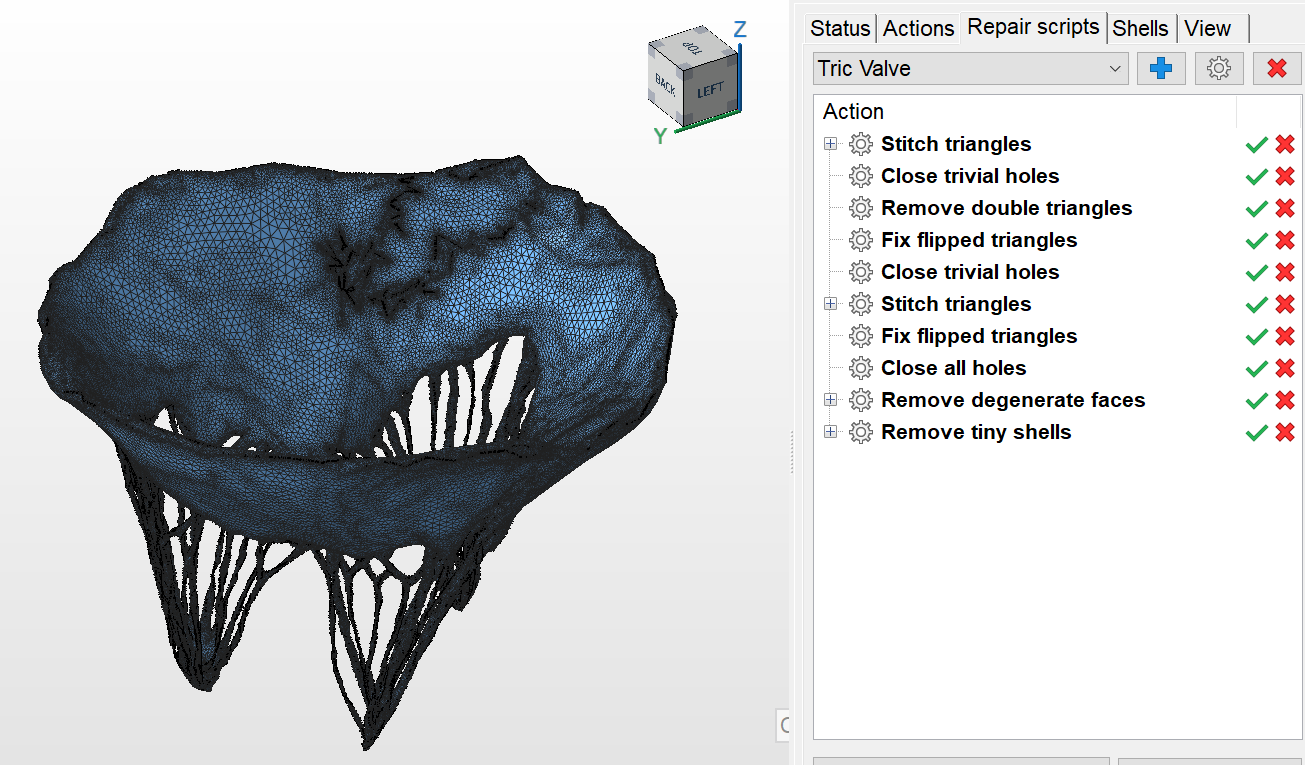
\includegraphics[width=0.8\textwidth]{figures/NetFabbRepair.png}
          \caption{Netfabb Repair Scripts}
          \label{fig:NetfabbRepair}
        \end{figure}
  \item Shell
        \begin{figure}
          \centering
          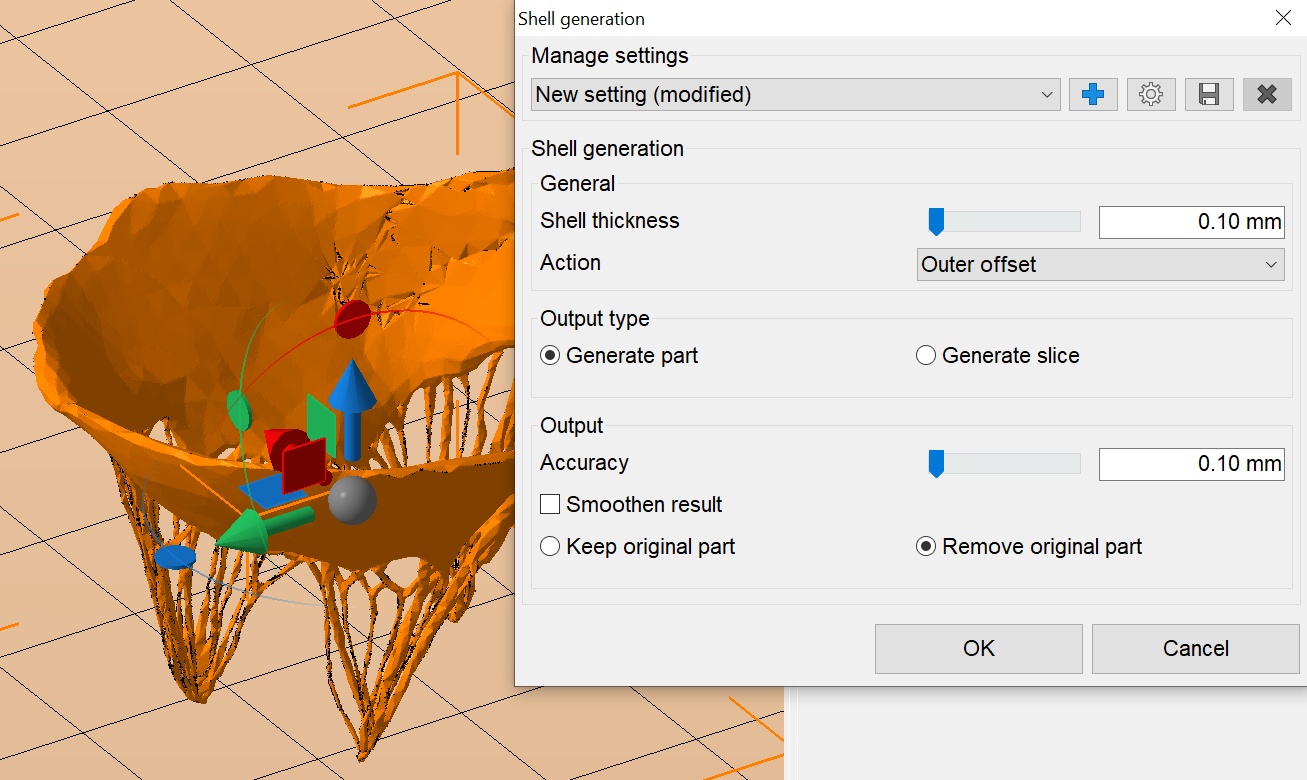
\includegraphics[width=0.8\textwidth]{figures/NetFabbShell.png}
          \caption{Netfabb Shell}
          \label{fig:NetfabbShell}
        \end{figure}
\end{itemize}


After the repairing and hollow shell process was completed the model was imported into Blender, here

Meshmixer was used in tandem with blender as it contained a very useful thickness analysis tool which could be used to see the varying thicknesses of the leaflets in the imported model, then Blender was used to manually edit the model using its sculpting tools to either thicken or thin the surface where appropriate.



% Physical prototyping:

% Printing errors
% Moulding errors
% Material errors
% Assembly errors
% Design errors


% Tools:

% 3D printer
% Spatula
% Syringe
% Precision blade
% Sanding paper
% Pliers
% Tweezers
\section{Prototyping}
\subsection{Valve Iterations}
\newthought{Preliminary Prototyping Methods}
The prototyping method went through a few key stages, throughout the simplified valve modelling stage the running methods were creating \gls{PLA} prints of the flat and balloon valve models and then using a silicone mould to capture its likeness, through feasability testing it was found this method was not suitable for reasons;
\begin{itemize}
  \item Silicone moulds could not hold firm enough in casting to maintain sub 1mm thicknesses
  \item The mould release agent was less effective on PU-Silicone interfaces than expected \todo{acronym or sidenotes}
  \item The moulds even with appropriate ventilation would still have air bubbles and not fill out to the edges of the part.
\end{itemize}
As it seemed no amount of optimization of this method would improve results further work was done to find a more suitable method.

\newthought{Press Moulding}
This new method involved designing blocks in SolidWorks as a separate body to the valve part and using the 'Combine' tool to subtract the valve part. This hollowed block could then be split in the middle to create a two-part mould.

The \gls{PU} resin \todo{acronym} could then be poured into the cavity part and the lid part pressed ontop with a C-clamp to create a tight seal.

Some key considerations developed over trial and error for this method were:

\begin{itemize}
  \item Embossing and debossing key slots to ensure the moulds could be aligned correctly.
  \item Sanding down the \gls{PLA} prints to a smooth finish so in combination with a tailored mould release the casted part could be separated easily.
  \item Utilizing a vacuum chamber to remove air bubbles from the resin before curing.
\end{itemize}

% Materials used:

% Platinum cure silicone
% Polyurethane resin
% Ecolex transparent silicone
% Epoxy
% PLA
% SLA resin
% B7000 adhesive
% Nylon write
% Mould release
% Grease
% Isopropyl alcohol
\section{Chordae Tendineae }
Initial conceptualization of the chordae tendineae involved having the valve as one homogenous material with the tendineae attached within the mould. However, as the project progressed and the complexity of the valve increased, it was decided that the tendineae should be a separate part that could be attached after the valve was cast. This was decided on as the elastic modulus of the tendineae was vastly different as they function to be pulled taught to stop the leaflets from prolapsing.

\newthought{Design of Choice:}
A 0.1mm nylon fishing wire was chosen to represent the tendineae as it was thin enough to be completely collapsible and not interfere with the opening in the diastolic phase.

The attachment to the valve was the more challenging aspect, a few methods were considered and tested:
\begin{itemize}
  \item Suture patterns along the cusp of the leaflets.
        \begin{itemize}
          \item A short continuous suture was used to attach a few tendineae to the leaflets on a sample piece of \gls{PU} how on a gentle tensile test the suture ripped out as the \gls{PU} wasn't strong enough to hold.
        \end{itemize}
  \item Using a small hole in the leaflet to thread the tendineae through and then knotting it on the other side.
        \begin{itemize}
          \item This method also failed as the elasticity of the \gls{PU} made it so the knot would have to be \gls{PU} would rip anyway.
        \end{itemize}
  \item Embedding the wire in the \gls{PU} leaflets.
        \begin{itemize}
          \item While hopeful the embedding technique proved not feasible as the wire just slipped out, there was an attempt made with thick and thin layers of additional \gls{PU} but to no avail.
        \end{itemize}
  \item Gluing the tendineae to the leaflets with a cyanoacrylate adhesive.
        \begin{itemize}
          \item While this method showed initial promise as the adhesive was strong enough to hold the tendineae after seconds of curing, when 24 hours passed the adhesive would harden much stiffer and deform the leaflets making them very rigid.
        \end{itemize}
  \item Gluing with B7000 adhesive.
        \begin{itemize}
          \item The B7000 adhesive was chosen as it was a flexible adhesive, initial tests werent fruitful but if left to set fully over 24 hours the bond became very strong and the leaflets retained their flexibility while also only needing a miniscule amount for a good hold so the very thin thickness of the leaflets wasnt negated.
        \end{itemize}
\end{itemize}
\section{Fixturing}
The ideal design criterion was considered carefully before modelling the test fixturing. The main desired outcomes from the testing that the fixturing should facilitate were:

\begin{itemize}
  \item The chordae tendineae should have fixed anchors which are fully adjustable axially and angularly.
  \item The valve should be able to be mounted in a way that the leaflets are not obstructed and the valve can be viewed from all angles for through evaluation.
\end{itemize}

\newthought{Design of Choice:}
A combination of 3D printed parts, off-the-shelf components and hand-cut threaded rods were used to emulate the initial sketch of the rig

The threaded rods allowed for the anchoring points of the tendineae to be adjusted axially.

Attached to the rods was the ring system with notches that could be adjusted angularly which the mock tendineae were passed through and fastened to with a rubber wedge.
\chapter{Experimental Setup and Testing}\label{ch:testing}
% \openepigraph{Everything in its right place \\
% There are two colours in my head}{Radiohead \textit{Everything In Its Right Place}}
\vspace{-2.5em}
% \newthought{Synopsis}\synopsisMethod

\mynewline
After completing the literature review I decided to go down two main paths: developing a representative valve and a anatomical valve. The representative valve would be a simple model that could be used to test the simulator and the anatomical valve would be a more complex model that could be used to test the simulator and also be used for educational purposes.

\section{Fixturing Assembly}

\section{Rig Assembly}

\section{Challenges and Mitigations}

\begin{itemize}
    \item Leakage: The pulsatile flow loop is a closed system, so leakage has to be carefully monitored. With the nature of the proof of concept rig containing many adapters and connections, it is important to ensure that all connections are secure and that there are no leaks. This was managed with the liberal use of teflon tape and tight fit Buna O-rings. Where there were still leaks, small containers was used to catch the fluid and pour back into the circuit.
    \item Air bubbles: Air bubbles greatly obstructed the coaptation of the valve leaflets. Interupting the fluid flow and also obscuring the view of the valve for evaluation of the coaptation. With the leaks in the system allowing air to enter repeated purging of the system was required to remove air bubbles with a syringe and tube entering through the proximal end of the system.
    \item Chordae Tendineae Adhesion: The adhesion of the most recently attached mock tendineae to the \gls{PU} leaflets had not fully set before the testing began. This resulted in the one of the tendineae detaching during coaptation. As the valve was still functioning the testing was not stopped to mitigate this issue.
\end{itemize}



\section{Biocompatibility}

\begin{fullwidth}
  \part{Results, Analysis, and Discussion}\label{pt:ResAnDis}
\end{fullwidth}
\parttoc[n]
\chapter{Results}\label{ch:results}
% \newthought{Synopsis}\synopsisMethod
The results of the testing of the proof of concept rig are presented in this chapter. The results are presented in a qualitative manner as the rig was not designed to provide quantitative results.
The goal of the testing was to determine if the proof of concept rig was able to simulate the coaptation of the tricuspid valve and the flow of blood through the valve, if the valve leaflets and chordae tendineae could sustain the systolic pressure developed from coaptation, verifying the functionality of the valve for use in the right-heart simulator and later integration of CroiValve DUO.

\section{Pilot Tests}
The teflon tape worked very well where applied however the 3D-printed end cap of the core testing chamber leaked a lot even after an attempt to seal with tack. This was due to a mis-fitting of the O-ring used on the part.

\section{Coaptation Test}
\newthought{The valve} part coapted well, septal and posterior leaflets in particular, the cusp of the anterior leaflet however didnt coapt with either of the adjacent two creating a larger regurgitant orifice than expected. This is likely due to;
\begin{itemize}
    \item The material properties of the \gls{PU} used not being elastic enough.
    \item The thickness of the leaflets being too thick making them less flexible.
    \item The overlapping length of nylon wire on the leaflets making them stiffer.
    \item The natural saddle shape of the valve annulus being flattened off to fit in the seating fixture.
    \item Leaflets length loss from the processing of the valve model.
\end{itemize}

\newthought{The chordae tendineae} held up well under the pressure and prevented the valve from prolapsing. They were tensioned to a point where they valve were allowed to partially prolapse similar to how native \gls{TV}'s do in regurgitant cases and an expected degree of prolapse occured as a result.

During assembly one of the chordae on the posterior leaflet broke leaving just two although this didn't majorly effect test results.

\begin{figure}
    \begin{fullwidth}
        \centering
        \subfloat[Head-On View]{%
            \href{https://drive.google.com/file/d/1epMX5xH8P03QeNA2DaLtc610iFQK58KK/view?usp=sharing}{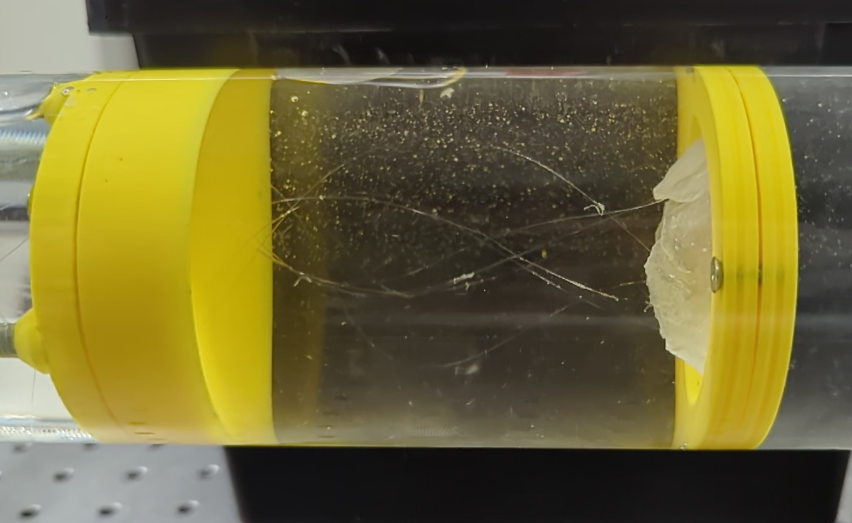
\includegraphics[width=0.45\linewidth]{figures/valverigcloseup}}%
        }\quad
        \subfloat[Oblique View]{%
            \href{https://drive.google.com/file/d/1RXlcIPh9iO5SNXvG8wYL6XBqwaXyd4fS/view?usp=sharing}{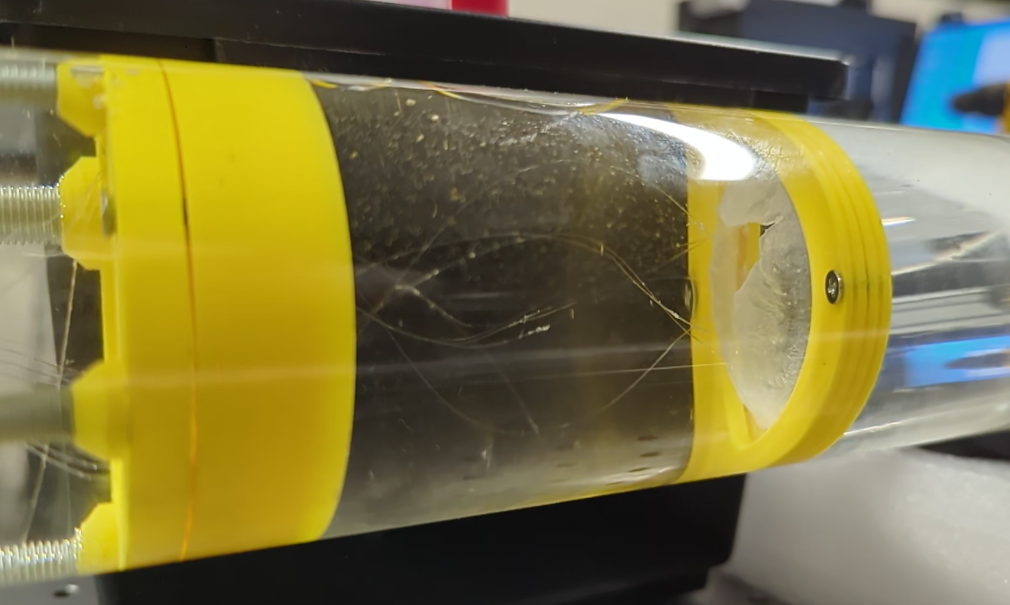
\includegraphics[width=0.45\linewidth]{figures/valverigcloseup2}}
        }
        \caption{Frame from video of valve coapting during testing \textbf{(click to view video)}}
        \label{fig:Videos}
    \end{fullwidth}
\end{figure}
\chapter{Discussion}\label{ch:Discussion}\addtocontents{lof}{\protect\contentsline{chapter}{\protect\numberline{\thechapter}Discussion}{}{}}
\newthought{Synopsis}\synopsisDiscussion

\section{Challenges and the Various Explored Approaches}
\subsection{Modelling Challenges}
\newthought{Mould Die Design}\\
The challenges in the early stages after deciding to work off of an pre-constructed anatomic valve geometry spawned many issues, it didn't allow for feature interaction in SolidWorks which prompted some very suboptimal prototyping choices that ended in a huge amount of time investment for an avenue that was eventually made obselete upon later findings. The series of 2-stage epoxy moulds developed as discussed in \cref{fig:moulddie} had a 72 hour curing time, which made the turnaround for learnings much slower to implement.

This process became obselete when the SolidWorks package being used was arbitrarily updated. It was discovered that the 'Segment Mesh' tool previously attempted to use to convert the STL to mesh body and then to a solid part had been overhauled to allow more complex geometries to be segmented. On this discovery the part was successfully converted to a solid body which allowed for it to be subtracted from an encompassing cylindrical body as originally theorised which was then split into the what were the foundations of the final design press mould pieces.

From this point further iterations of the press mould were much quicker, taking only 4-5 hours, reducing the print-to-casting time by 95\%. 20 hours for finalised designed where the layer lines were much smoother, being almost invisible on the casted part.
\begin{figure}[H]
    \centering
    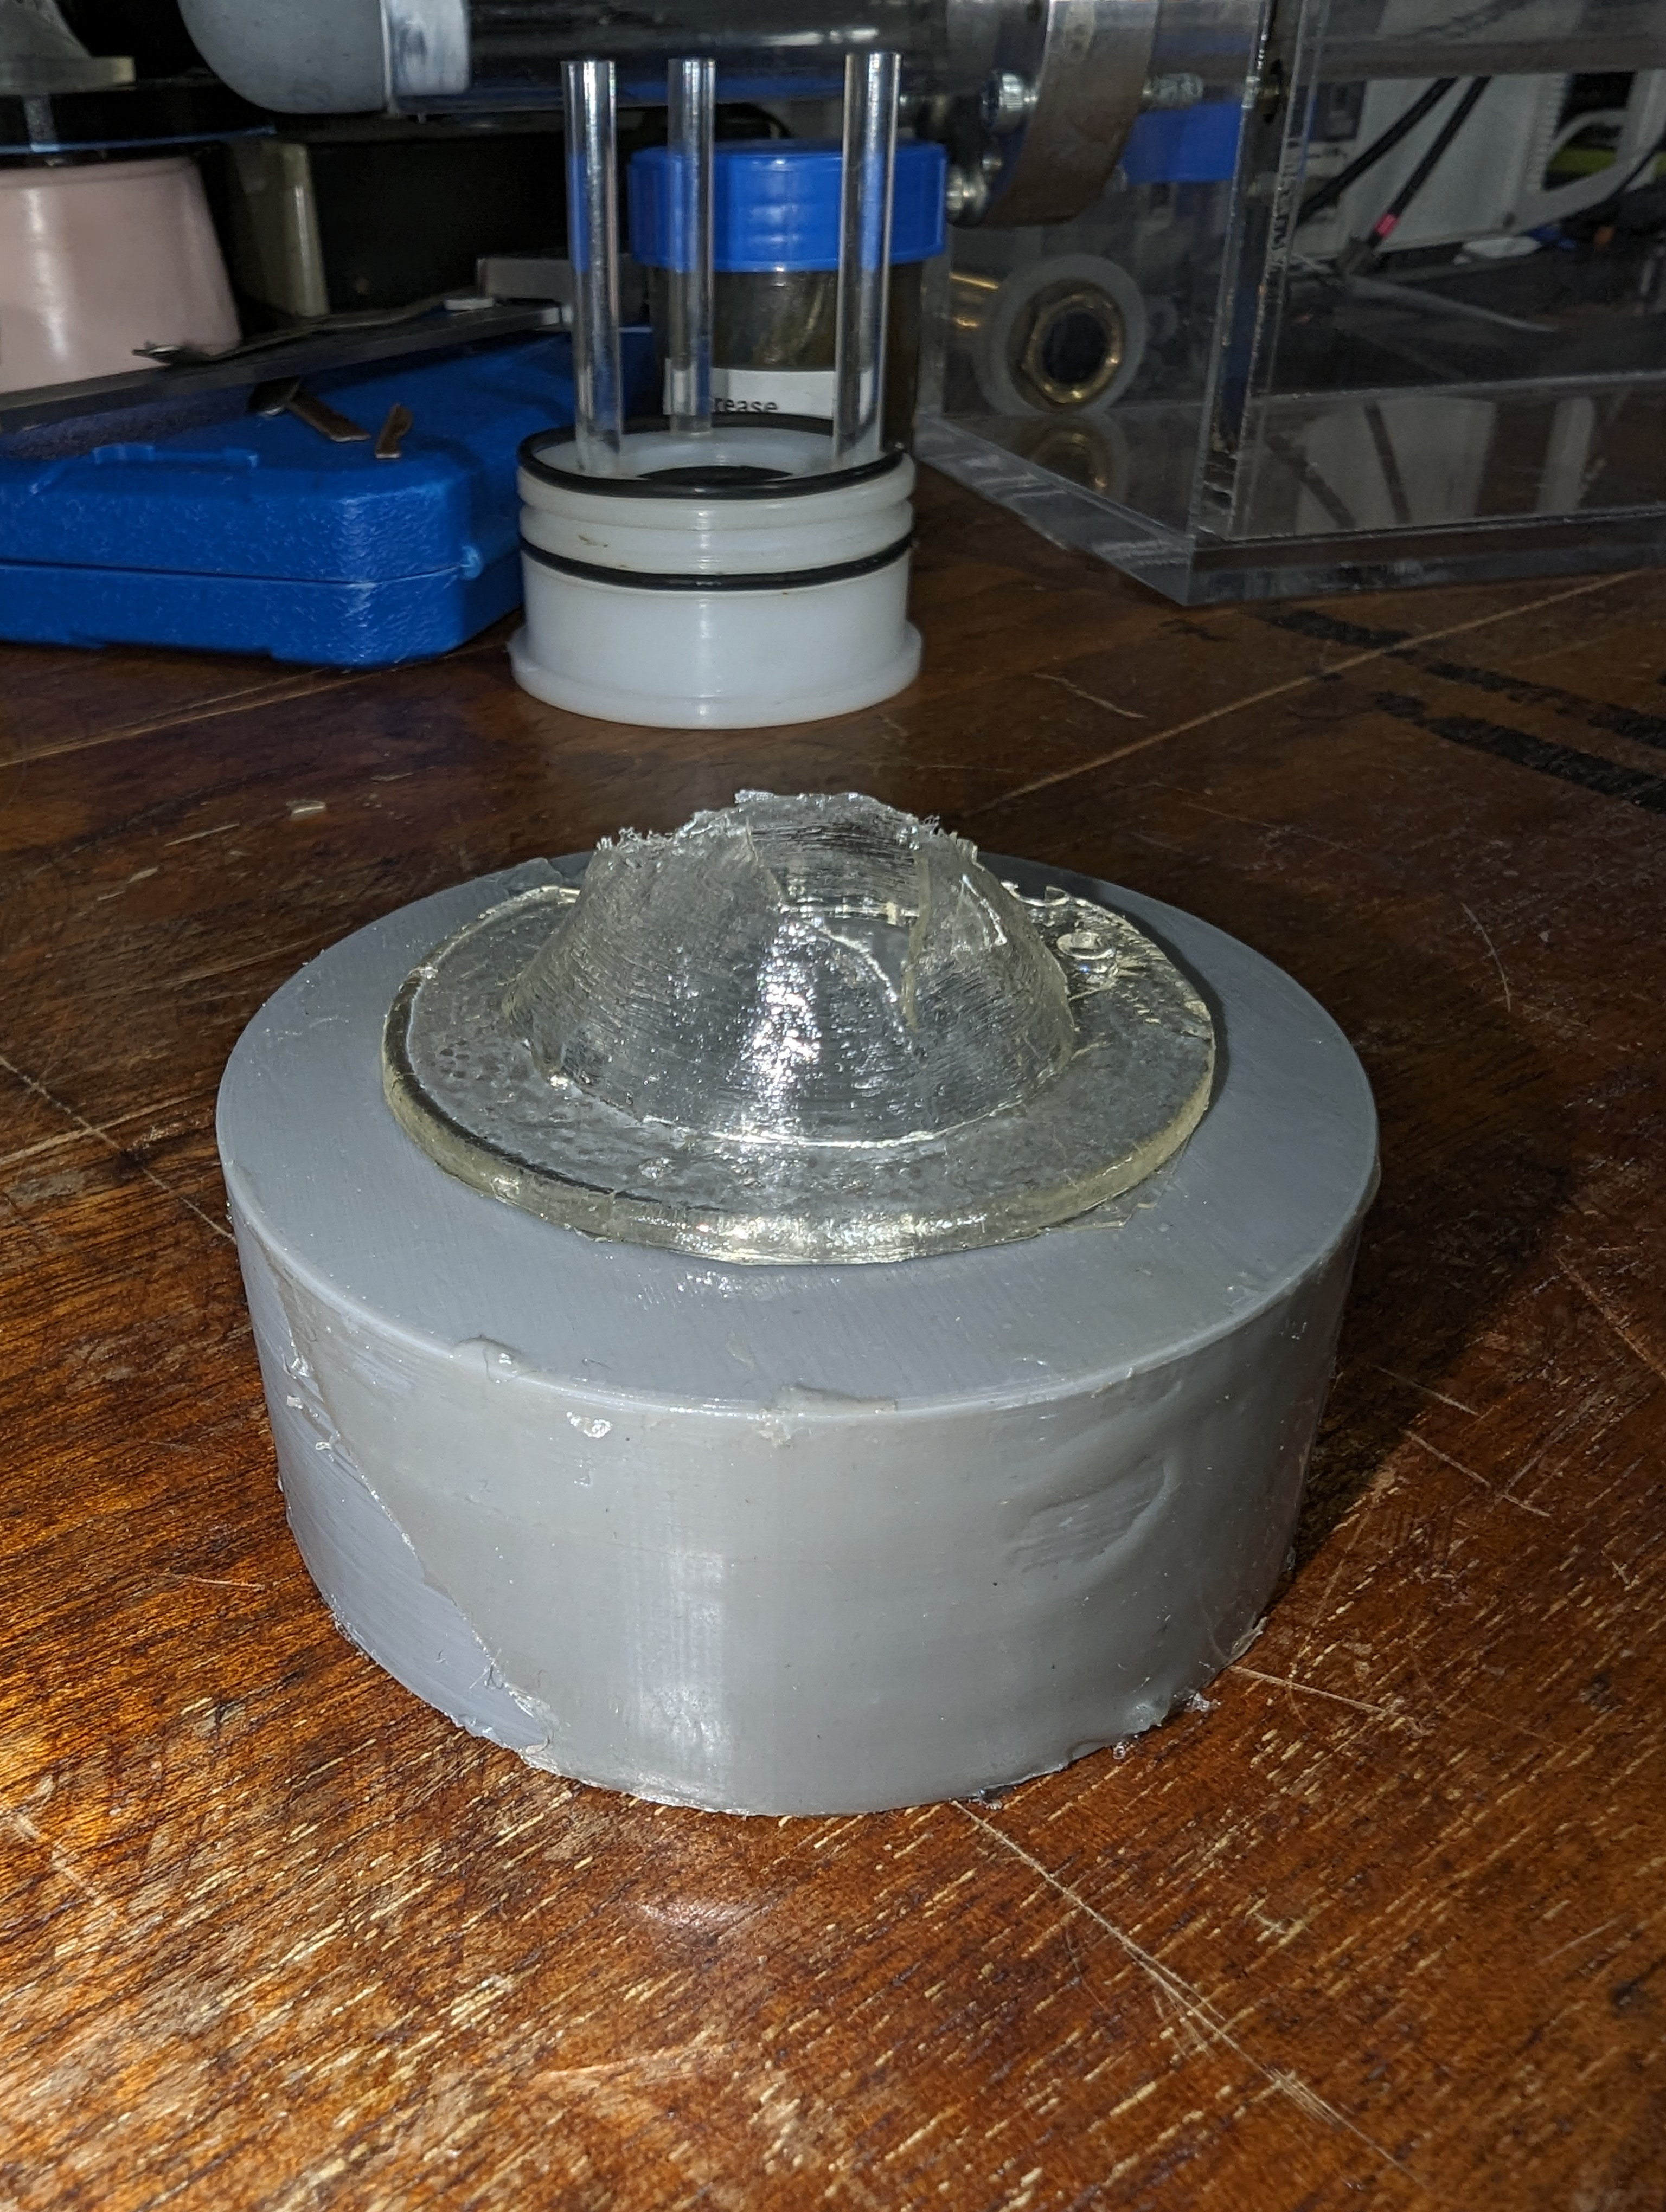
\includegraphics[width=0.75\textwidth]{figures/latercastnice.jpg}
    \caption{Final cast of anatomical valve}
    \label{fig:cast1}
\end{figure}

\newthought{Valve Design}\\
Another area that caused an excess of time used was the post processing of the anatomical valve geometry, in becoming acquainted with STL modelling\sidenote{Software packages like blender use mainly sculpting tools that are used to modify the surface as opposed traditional CAD programs like SolidWorks where parts are built up from a tree of features} on the various programs trialed throughout the study the model was transferred across systems a lot to utilize the different tools each had, for example, how blender had great scuplting tools but lacked simple geometry analysis which was required for monitoring the surface as the thickness was homogenised.

While blender has capabilities to manipulate shaders to render this kind of information however due to it being an opensource program the process of developing a custom shader for this purpose was deemed too rescource intensive however if further work was conducted with many patient-specific models being developed it would be quite likely the most efficient option.

\subsection{Manufacturing Challenges}

\newthought{Chordae Tendineae Prototyping}\\
The tendineae attachment to the leaflets was another highly contested and thought out factor of the design. Balancing the rigidity that is added to the leaflets by some methods in attaching the nylon wire and the adhesion to the leaflet is very dificult, for the scope of this study it was found that B7000 adhesive worked well as the tendineae could be effectively attached with minimal disruption to the mechanics of the valve however this did add thickness to the leaflets which not only adds rigidity that hinders coaptation in experimental use but also brings many issues for potential computational simulations that could be conducted in tandem to a study of this nature.

Studies like \citeonly{karlExvivoInvitroDynamic2024} which had been examined in the later stages of the study use a method of embedding their chordae tendineae within the leaflets, containing a medical gauze matrix, so that the tendineae do not detach under tensile forces. An approach like this could prove very effective in application to this study as it would simplify the manufacturing process in that with a the tendineae can be attached to the gauze matrix prior to \gls{PU} casting ensuring accurate and replicable placement.

\newthought{Valve Prototyping}\\
The prototyping conducted through the study for the mould parts, fixturing and experimental rig revealed a few key insights into the rapid-prototyping landscape. For each print the configuration of the printer was tailored to the purpose of the parts being produced, parts being made in early iterations were set to a faster infill and layer height setting, whereas finalised ideas were set to slower, higher resolution settings.

It was found these dense high definition settings needed for aaccurate and rigid mould die had issues of their which took many iterations and failed prints to perfect. They often resulted in a large amount of stringing, a printing defect, which in many cases was not solvable via post processing. To circumnavigate this the researchers in the UCD print lab were consulted. Tailored settings in Prusa Slicer were then programmed for the geometry where the resulting gcode would stop the nozzle from crossing the perimeter of the valve moulds, retraction settings would stop the printer from leaving blobs of plastic on the interior of the mould and z-axis seams were alligned to not interfere with the geometry.
\mynewline
In earlier stages of the study a resin \gls{SLA} printer was used to manufacture an anatomic model for the silicone mould method discussed in \cref{fig:silimould} which however it was not feasible to develop further iterations from resin due to the printer being in a separate lab and having a much higher cost of with proprietary resins. Two major benefits to \gls{SLA} printing are;

\begin{figure}[H]
    \centering
    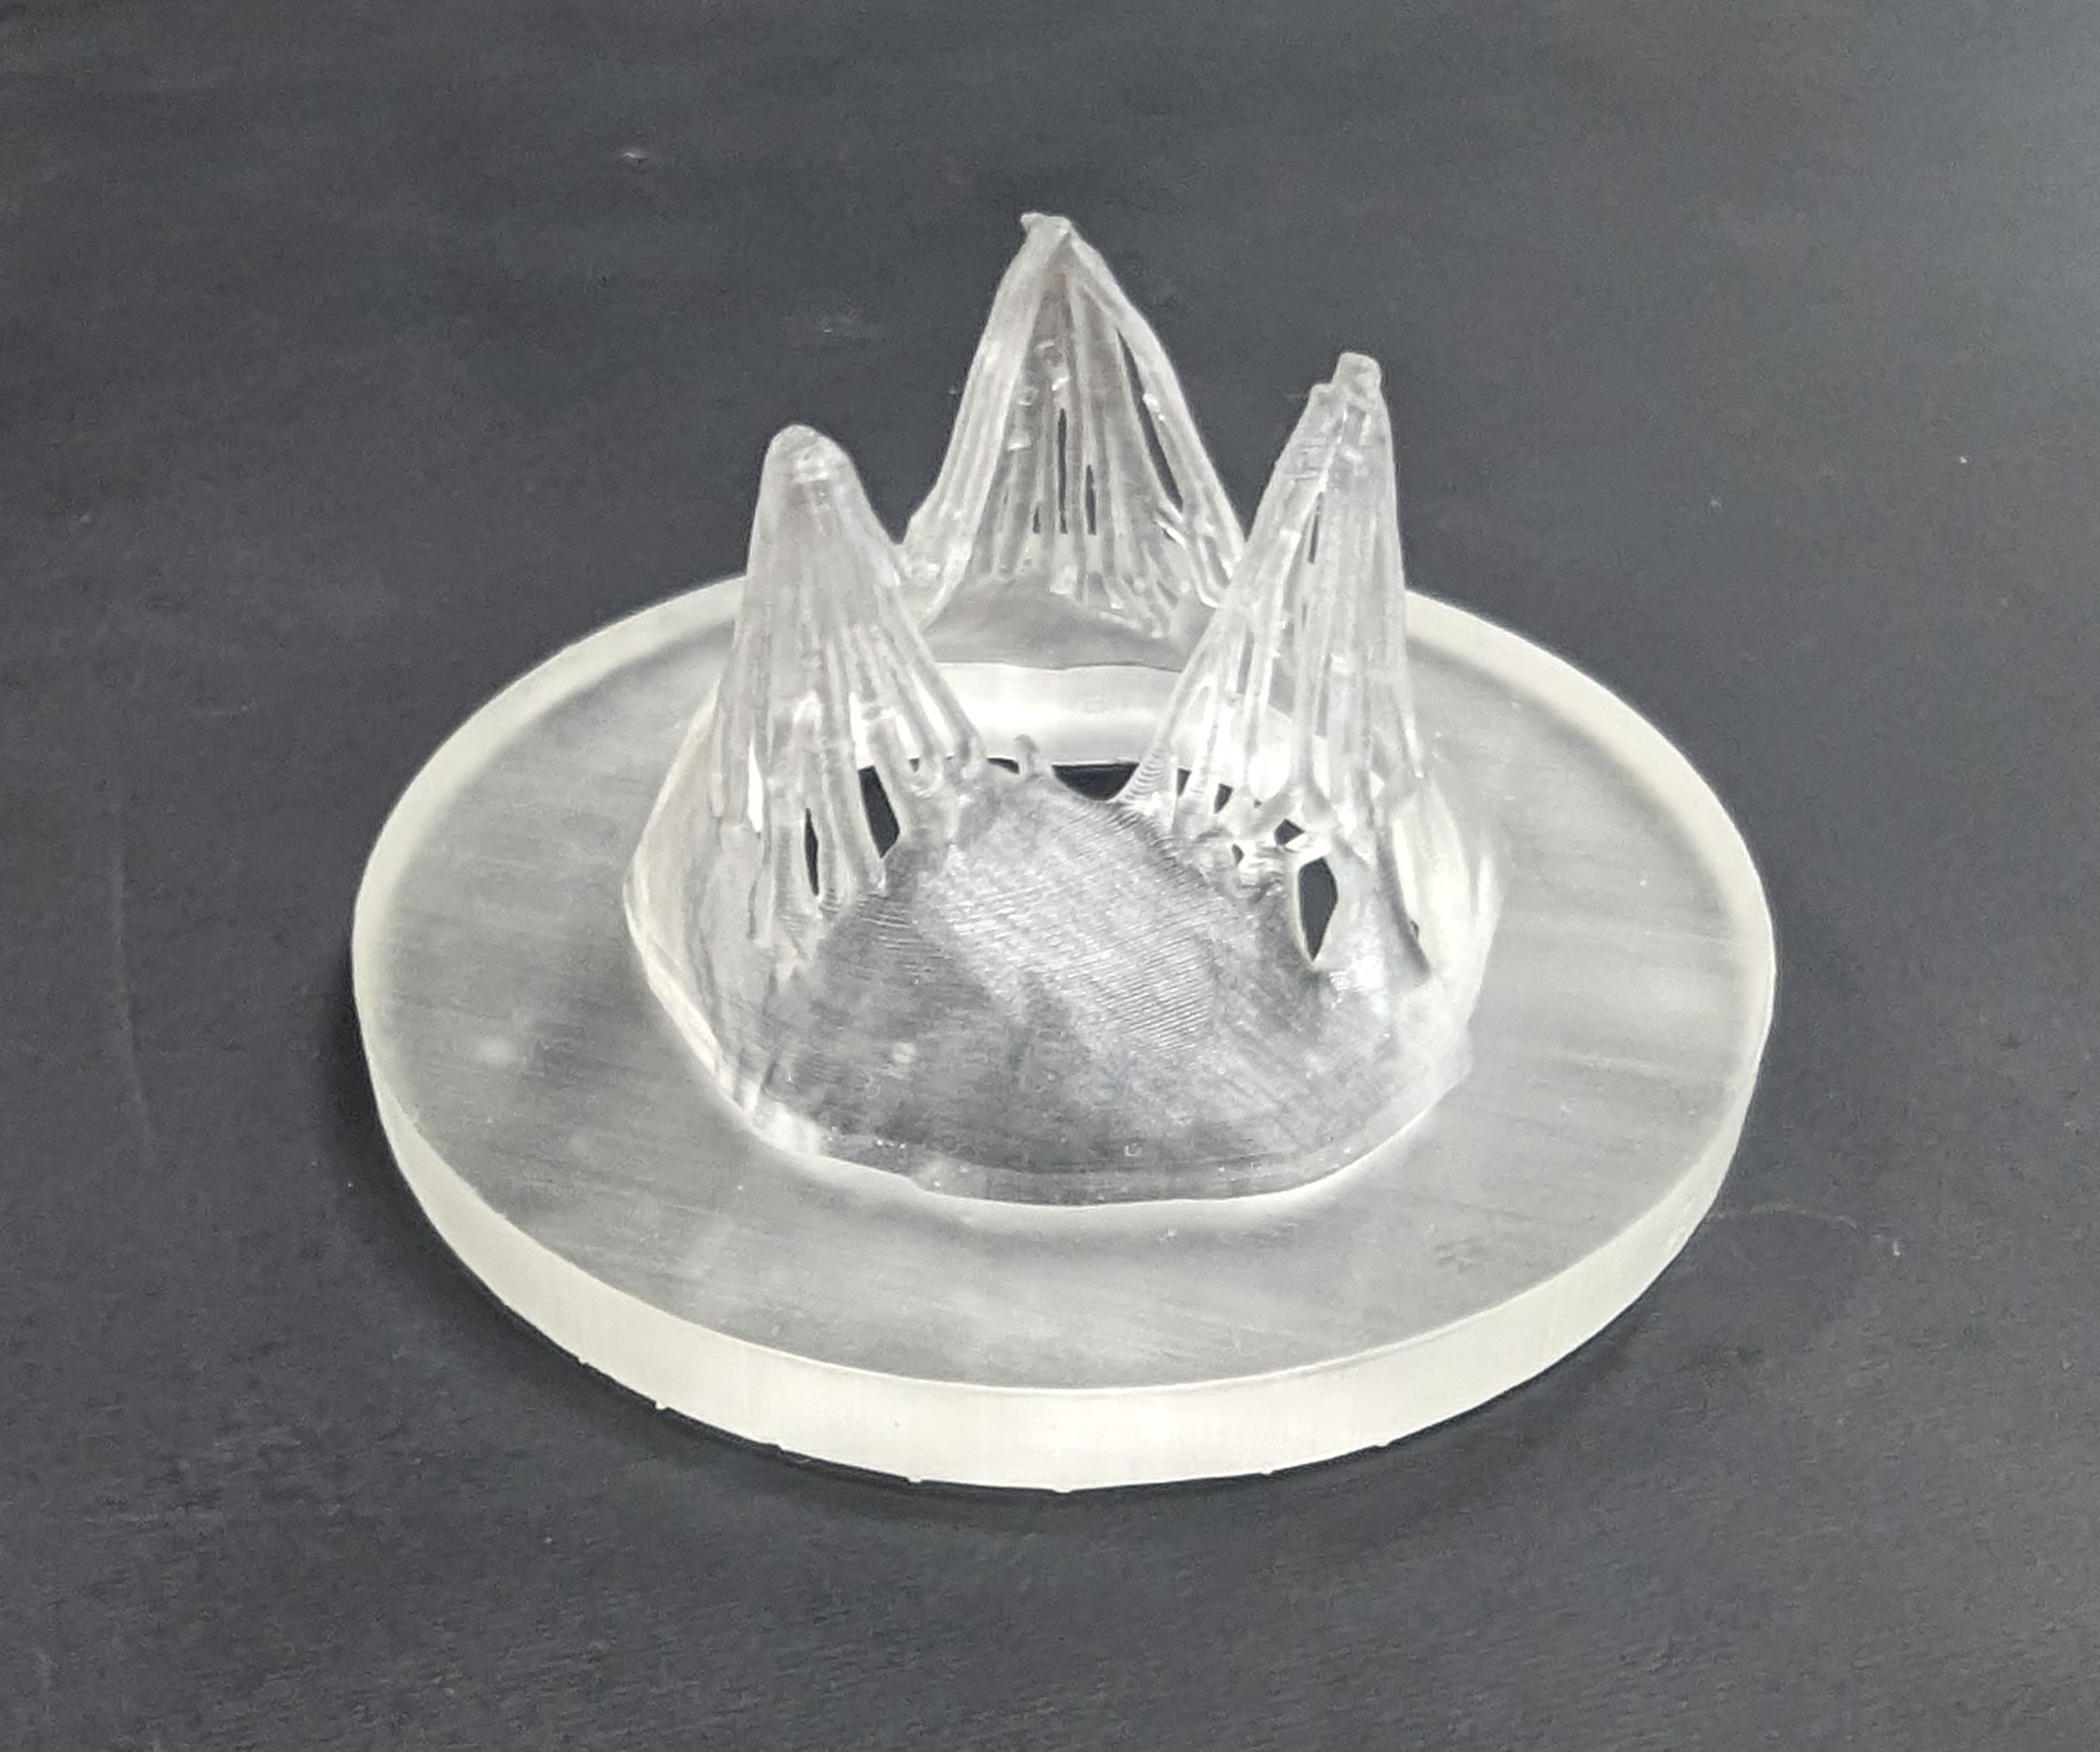
\includegraphics[width=0.75\textwidth]{figures/resinprintanat.jpg}
    \caption{Early revision \gls{SLA} print of anatomical valve}
    \label{fig:reso}
\end{figure}
\marginpar{\textbf{Resources:}
    \begin{itemize}
        \item \href{https://help.prusa3d.com/article/faq-frequently-asked-questions_1932}{Prusa TDS}
        \item \href{https://formlabs.com/blog/understanding-accuracy-precision-tolerance-in-3d-printing/}{FormLabs TDS}
    \end{itemize}
}
\begin{itemize}
    \item The vastly increased tolerance of resin printing\\
          Prusa \gls{FDM}:0.3mm\\
          FormLabs \gls{SLA}:0.01mm
    \item The reduced layer height that resin printing is capable of\\
          Prusa \gls{FDM}:0.05mm\\
          FormLabs \gls{SLA}:0.025mm
\end{itemize}
This has two main benefits regarding this study;
\begin{itemize}
    \item Minimizing layer height results in mould parts reduces surface affects
    \item Reducing adhesion of cast part to mould, this is minimized on \gls{PLA} parts with mould release and sanding however with casted parts on this degree of thickness there can still be an increased risk of breakage in the demoulding process.
\end{itemize}
Another option worth considering is machining from either steel or a performance plastic like delrin \citeonly{liProcessOptimizationInmold2022}, this would be more expensive however it could be worth the cost for moulds that need to be used for a larger number of castings as well as increasing the precision over multiple casts since you the 3D printed parts can warp under the pressure of the clamping. The transparency of the part was a consideration for further work on the valve as the proposed integration into the right heart simulator would involve \gls{PIV} measurement where maintaining transparency would allow for an measured flow field uninterrupted by the valve, this was an issue in studies like \citeonly{rabbahNovelLeftHeart2013} and the efficacy on dynamic transparent parts in \gls{PIV} rigs has been shown in studies like \citeonly{busenDevelopmentVitroPIV2017}

\section{Contextualizing Results}

% Discuss how your results relate to previous studies and theoretical frameworks. Are your findings consistent with other studies, or do they diverge?
% Analyze the significance of any discrepancies and explore possible reasons.

The results of this study have shown how development of imitative synthetic heart valves can be a valuable tool in cardiac simulators. The coaptation tests on the valve show great promise for technology of this nature, previously in simulational studies such as \citeonly{rabbahNovelLeftHeart2013} dissected porcine valves, \citeonly{gintyModelingPatientSpecificDeformable2018} used rigid valves and \citeonly{raghavExperimentalAssessmentFlow2018} non-anatomically representative valves which each have major limitations in their ability for a wider range of experiments.\\
Some such limitations of these valves which the work of this study has surpassed are;
\begin{itemize}
    \item The longevity of porcine for repeated experiments. While it can be stored in the likes of formalin the tissue degrades over time which leads to an irrepeatability in testing and eventual need for replacement.
    \item Semi-rigid valves can't be used in flow studies as they can't deform to coapt.
    \item Non-anatomical valves can coapt but don't represent true geometry which won't yield accurate results.
\end{itemize}

\newthought{Chordae Tendineae Performacnce:}\\
The coaptation test illustrated how the chordae tendineae can be used in a synthetic part to prevent prolapse and aid coaptation. The aligns well with how it had been done before such as in \citeonly{rabbahNovelLeftHeart2013} and \citeonly{karlExvivoInvitroDynamic2024} where native and synthetic tendineae were used respectively. Such works also show how this part of the model can be manipulated with motors to simulate the contraction of papillary muscles which while not applicable to the current design of the right heart simulator, could be developed for future iterations or simpler rig design like that of the tube-based coaptation test \cref{fig:Videos}

\newthought{Leaflet Performance:}\\
The area with most room for improvement is likely the leaflets. The final iteration from this study came very far relative to the initial iterations in term of rigity, transparency and geometrical precision, it also performed better than similar attempts from other studies like \citeonly{gintyModelingPatientSpecificDeformable2018} although in regards to the initial design criteria from section:\cref{sec:Design Criteria}  it is lacking in functional performance and scalability

Not all the leaflets coapted together which was the objective however it was supposed to occur from annulur dilation and chordal loosening not from just the geometry, this is most likely due to the model of the valve being based off a valve in the diastolic phase so the full length of the leaflets was malformed in \gls{CT} conversion as they weren't not being under load from the presuure. This can be seen in \cref{fig:Videos}:B where the leaflets do move back but are not long enough to meet eachother. The work of \citeonly{karlExvivoInvitroDynamic2024} capture this well in their mitral valve design, they did well with leaflet length however theyre design was not anatomically representative, building off this to capture both physiological replicity and functional performance would be a first of it's kind for in-vitro tricuspid valve testing.






\begin{fullwidth}
  \part{Epilogue}\label{pt:epilogue}
\end{fullwidth}
\parttoc[n]
\chapter{Conclusions and Future Work}\label{ch:conclusion}\addtocontents{lof}{\protect\contentsline{chapter}{\protect\numberline{\thechapter}Conclusion}{}{}}
\section{Conclusions}
In this thesis, a mock tricuspid valve was developed to improve the accuracy and functionality of right heart simulators. Through careful design and development, a model was created that accurately replicates the anatomical and biomechanical properties of the natural tricuspid valve and integrates effectively with existing simulation systems.

Challenges related to material compatibility and complex valve dynamics were addressed through advanced material testing and iterative design modifications. A prototype was produced, setting a new standard for realistic and functional heart valve simulators and potentially improving patient outcomes in cardiac care.

This work establishes a foundation for future research, suggesting further innovations in material technology and dynamic simulation capabilities. The anticipated integration of sophisticated computational models and exploration of new materials is expected to advance the capabilities of heart valve simulators significantly, bridging the gap between theoretical research and clinical application, and advancing biomedical engineering in cardiac care.

\newthought{In conclusion,} this study shows how the design process can be fraught with many more obstacles of many more varieties than expected. It resulted more in learnings of the iterative process of design and prototyping compared to test method development than expected.
% The study resulted in a manufacturing process that is consistent and effective in producing anatomically accurate valve models, developed over many different approaches with the strengths taken from each and weaknesses phased out. It also resulted in a test method that was able to effectively test the basic efficacy of the produced valves in a controlled environment and potential to very easily be adapted to introduce a variety tricuspid valve medical devices with simple fixturing and also account for variables like; pressure, flow rate, flow field, and regurgitant characteristics like orifice and volume, once integrated with the right heart simulator.
% The implications this type of testing could have on the development of \gls{TTVR} devices is significant. The ability to test the efficacy of these devices in a controlled environment can provide important data that can influence design choices and potentially mitigate against the risk of device failure in the clinical investigations.

\section{Future Research Directions}
Briefly touched on in the discussion were a few areas that further development in this project is very promising, continuing to decrease valve thickness will likely yield even more representative results and weaving chordal attachments into the leaflets will improve repeatability of fabrication while also aligning models more closely to that of \gls{CAD} designs for computational models.

% Pressure monitoring during test, 36\% glycerin for blood viscosity - rabbah
% In vitro micro ct scanning
\begin{figure}[H]
    \begin{fullwidth}
        \centering
        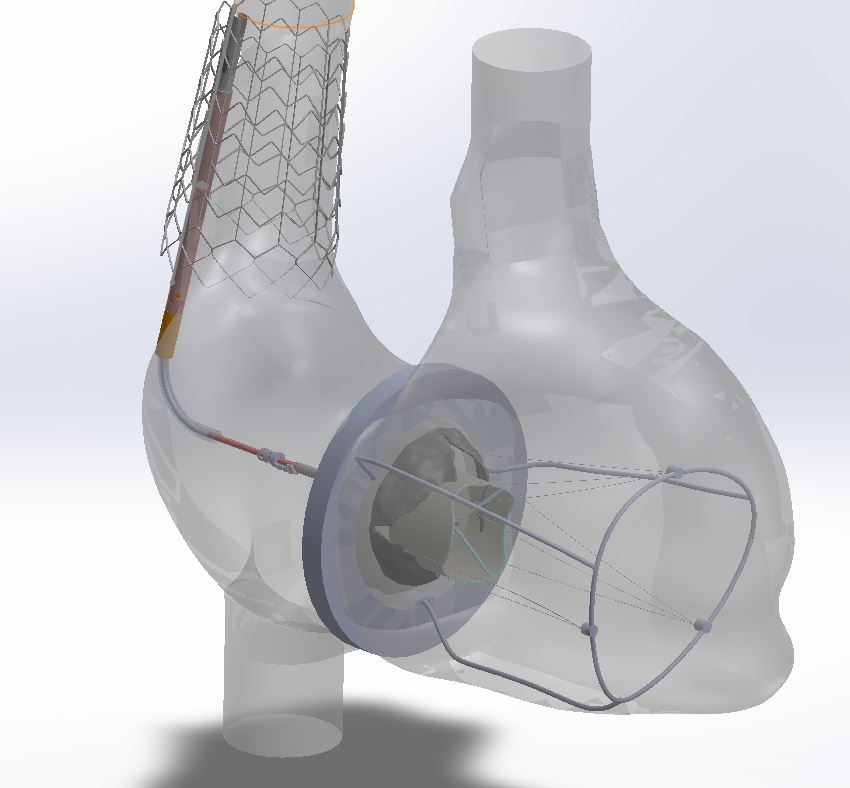
\includegraphics[width=0.8\textwidth]{figures/future}
        \caption{An assembly of the CroiValve DUO device in the right heart simulator}
        \label{fig:duo_assembly}
    \end{fullwidth}
\end{figure}
The next steps in this research will primarily be to fully integrate this valve into the right heart simulator. From there the rig be enhanced to involve \gls{TTVR} devices to characterize their efficacy on regurgitant valves. The main prospective device to integrate is the CroiValve DUO device which partially occludes the annulus of the valve reducing  regurgitant flow. While not reaching full fabrication due to time constrants, an assembly of what this would look like was created to illustrate how this would look. The models of the right heart simulator was used in designing the fixturing to them flush against the heart chamber for minimal flow disturbance.

Integration of the DUO device system could be carried out quite simply by implanting it aligning with the clinical procedure by anchoring the stent in the superior vena cava of the right heart simulator.

% At the moment the CroiValve team don't have the means to conduct work of this nature so the data collected in this study could be used to inform the design inputs of later interations.

% % === BACK MATTER ===% \backmatter{}
\chapter*{Appendix}\label{ap:appendix}

Solidworks drawings



% === BIBLIOGRAPHY ===

\clearpage
% \phantomsection
% \addcontentsline{toc}{chapter}{Bibliography}
\begin{fullwidth}
    \printbibliography{}
\end{fullwidth}

% 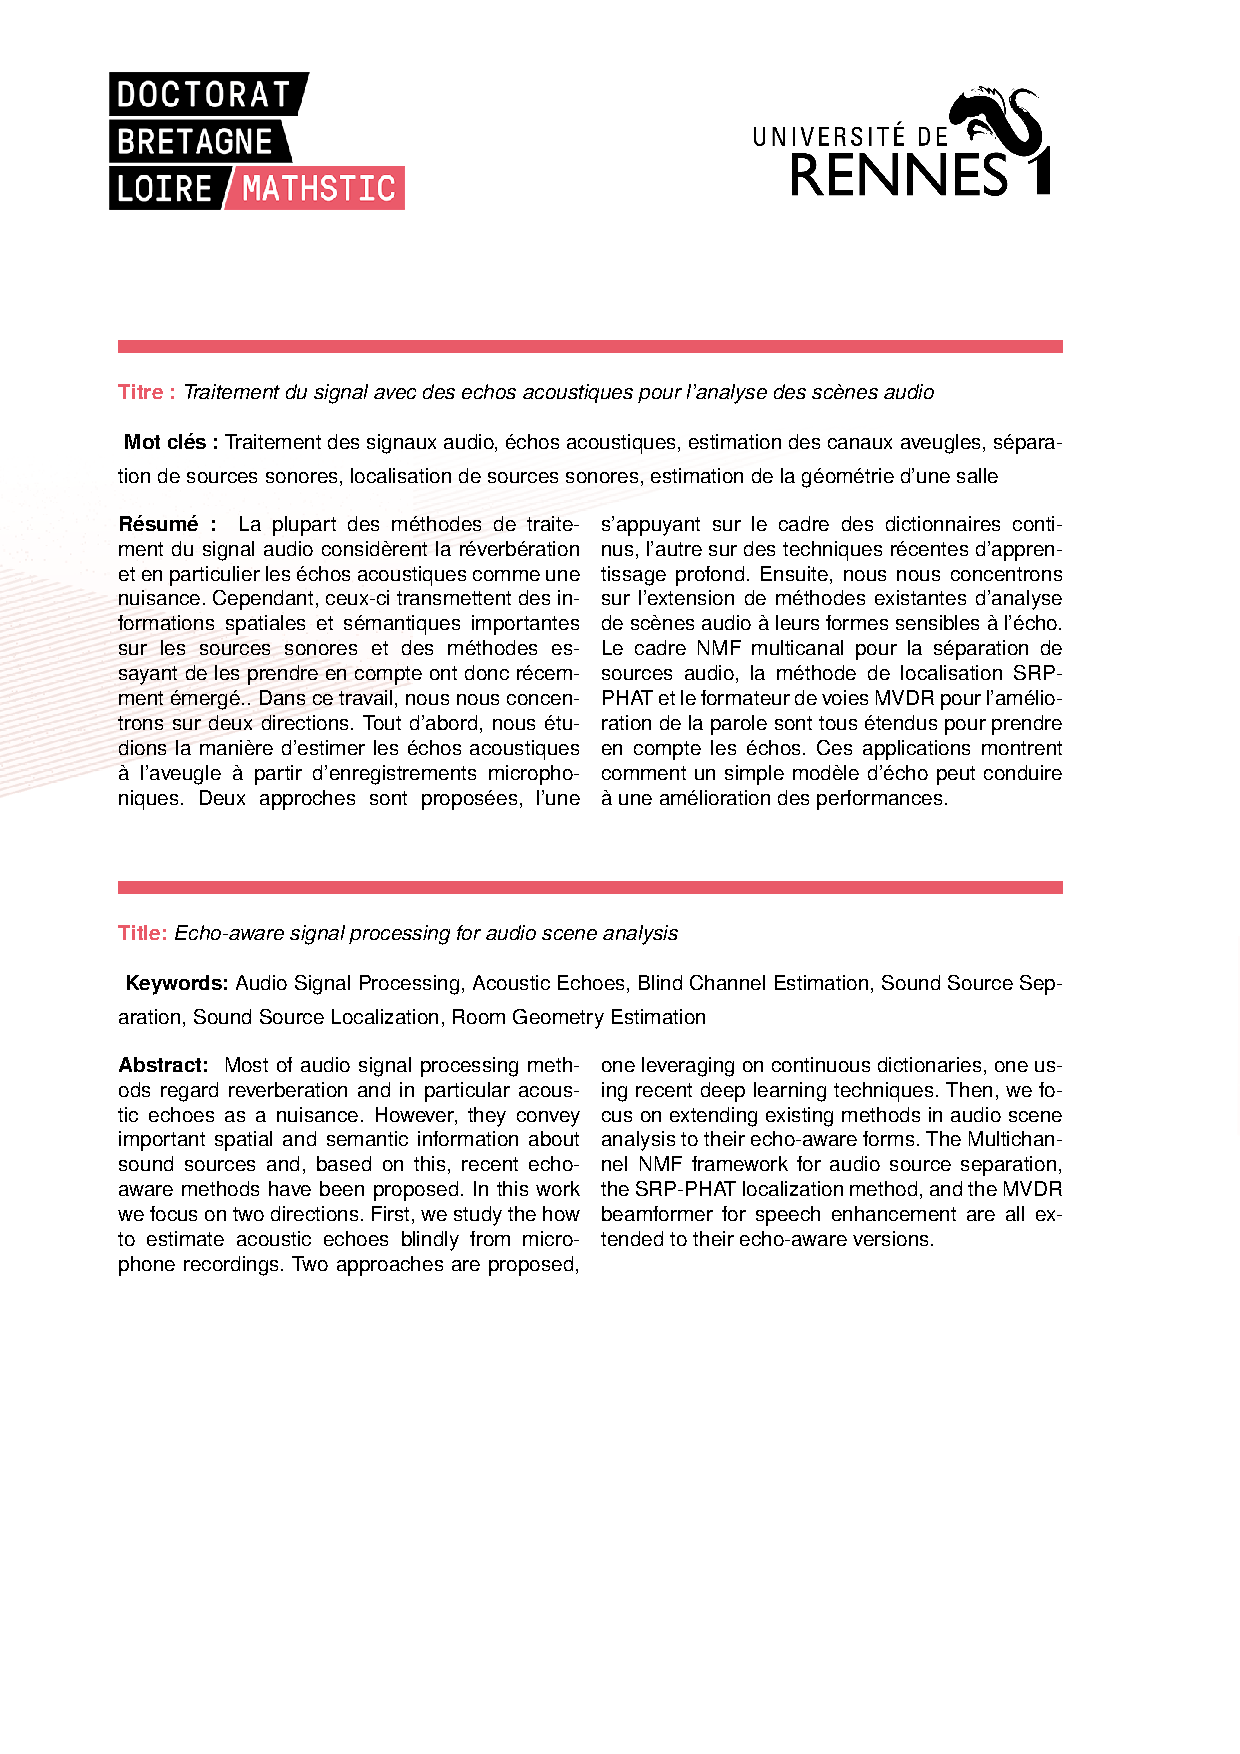
\includepdf{assets/last.pdf}

\end{document}